%&LaTeX
\documentclass[11pt,a4paper]{article}
\usepackage[frenchb,english]{babel}
\usepackage[applemac]{inputenc}
\usepackage[OT1]{fontenc}
\usepackage[]{graphicx}
\usepackage{amsmath}
\usepackage{amsfonts}
\usepackage{amsthm}
\usepackage{amssymb}
\usepackage{tikz}
\graphicspath{ {./figures/} }
%\input{8bitdefs}

% marges
\topmargin 10pt
\headsep 10pt
\headheight 10pt
\marginparwidth 30pt
\oddsidemargin 40pt
\evensidemargin 40pt
\footskip 30pt
\textheight 670pt
\textwidth 420pt

\def\imp{\Rightarrow}
\def\gcro{\mbox{[\hspace{-.15em}[}}% intervalles d'entiers 
\def\dcro{\mbox{]\hspace{-.15em}]}}

\newcommand{\be} {\begin{enumerate}}
\newcommand{\ee} {\end{enumerate}}
\newcommand{\deb}{\begin{eqnarray*}}
\newcommand{\fin}{\end{eqnarray*}}
\newcommand{\ssi} {si et seulement si }
\newcommand{\D}{\mathrm{d}}
\newcommand{\Q}{\mathbb{Q}}
\newcommand{\Z}{\mathbb{Z}}
\newcommand{\N}{\mathbb{N}}
\newcommand{\R}{\mathbb{R}}
\newcommand{\C}{\mathbb{C}}
\newcommand{\F}{\mathbb{F}}
\newcommand{\U}{\mathbb{U}}
\newcommand{\re}{\,\mathrm{Re}\,}
\newcommand{\im}{\,\mathrm{Im}\,}
\newcommand{\ord}{\mathrm{ord}}
\newcommand{\Gal}{\mathrm{Gal}}
\newcommand{\legendre}[2]{\genfrac{(}{)}{}{}{#1}{#2}}


\title{Solutions to David A.Cox  "Galois Theory''}

\refstepcounter{section} \refstepcounter{section}
\refstepcounter{section} \refstepcounter{section}
\refstepcounter{section}\refstepcounter{section}\refstepcounter{section}\refstepcounter{section}
\refstepcounter{section}\refstepcounter{section}\refstepcounter{section}\refstepcounter{section}
\refstepcounter{section}\refstepcounter{section}


\begin{document}



\section{Chapter 15 : THE LEMNISCATE}

\subsection{DIVISION POINTS AND ARC LENGTH}

\paragraph{Ex. 15.1.1}{\it Prove that the numbers described in Abel's theorem at the beginning of the chapter are precisely those in Theorem 10.2.1, provided we replace ``product of several numbers'' with ``product of distinct numbers'' in Abel's statement of the theorem.
}
\begin{proof}
The numbers described in Theorem 10.2.1 are the integers $n = 2^s p_1\cdots p_r$, where $p_1,\ldots,p_r$ are distinct Fermat primes, of the form $p_k = 2^{n_k} + 1$. Thus these numbers are the product of {\it distinct} numbers of the form $2^m$, or $2^{m}+1$, where $2^{m} + 1$ is prime, as described in the Theorem of Abel.
\end{proof}

\paragraph{Ex. 15.1.2}{\it Show that in polar coordinates, the equation of the lemniscate is $r^2 = \cos(2\theta)$.
}
\begin{proof}
By definition, a point $M = (x,y) \in \R^2$ is a point of the lemniscate $L$ if and only if
$$(x^2 + y^2)^2 = x^2 - y^2.$$ 
If $(r,\theta)$ are polar coordinates of $M = M(r,\theta)$, then $x = r \cos\theta, y = r \sin\theta$, thus, using $\cos^2 \theta + \sin^2 \theta = 1$, and $\cos(2\theta) = \cos^2 \theta) - \sin^2 \theta$, we obtain
\begin{align*}
M(r,\theta) \in L & \iff (r^2 \cos^2\theta + r^2 \sin^2\theta)^2 = r^2 \cos^2\theta - r^2 \sin^2\theta\\
&\iff r^4 = r^2 \cos(2\theta)\\
&\iff r^2 = \cos(2\theta).
\end{align*}
The equation of the lemniscate is $r^2 = \cos(2\theta)$.
\end{proof}


\paragraph{Ex. 15.1.3}{\it Prove that the two improper integrals $\int_0^1 (1-t^4)^{-1/2} \mathrm{d}t$ and $\int_{-1}^0 (1-t^4)^{-1/2} \mathrm{d}t$ converge.
}
\begin{proof}
 The map $t \mapsto (1-t^4)^{-1/2}$ is continuous on $[0,1[$, thus $t \mapsto(1-t^4)^{-1/2} \mathrm{d}t$ is summable on $[1,x]$ for all $x \in [0,1]$.  

Since $1-t^4 = (1-t)(1+t+t^2+t^3)$, $(1-t^4)^{-1/2} \sim [4(1-t)]^{-1/2}$ in the neighborhood of $1$. The Riemann Criterium shows that $\int_0^1 (1-t)^{-\alpha} \mathrm{d}t$ converges if  $\alpha  < 1$, and here $\alpha = 1/2$. Since $(1-t^4)^{-1/2} >0$, this is sufficient to prove that $\int_0^1 (1-t^4)^{-1/2} \mathrm{d}t$ converges.

Since $t \mapsto (1-t^4)^{-1/2}$ is even, the same is true in the neighborhood of $-1$, thus $\int_{-1}^0 (1-t^4)^{-1/2} \mathrm{d}t$ converges.
\end{proof}

\paragraph{Ex. 15.1.4}{\it  Prove the arc length formula stated in (15.6)}
\begin{proof}
 Here the equation of the ellipse $E$ is
 $$x^2 + \frac{y^2}{b^2} = 1,$$
 with eccentricity $k = \sqrt{1- b^2}$.

We compute the arc length $l$ of (E) between $x = u, y=v\ (-1<u<v<1)$ on the upper part of the curve. Then
$$l =  \int_u^v \sqrt{1+\left( \frac{\D y}{\D x}\right)^2}\  \D x,$$
where $y = f(x) = b \sqrt{1-x^2}.$ Then $f'(x) =  \frac{\D y}{\D x }= -\frac{2x}{\sqrt{1-x^2}}$, thus
\begin{align*}
l &=  \int_u^v \sqrt{1+\left(\frac{bx}{\sqrt{1-x^2}}\right)^2}\  \D x\\
&=\int_u^v \sqrt{\frac{1 - x^2 + b^2 x^2}{1-x^2}}\  \D x\\
&=\int_u^v \sqrt{\frac{1 - k^2 x^2}{1-x^2}}\  \D x\\
\end{align*}
We have proved
$$l =  \int_u^v \sqrt{1+\left( \frac{\D y}{\D x}\right)^2}\  \D x = \int_u^v \sqrt{\frac{1 - k^2 x^2}{1-x^2}}\  \D x = \int_u^v \frac{\sqrt{(1-x^2)(1 - k^2 x^2)}}{1-x^2}\  \D x.$$
The arc length of the ellipse is given by an elliptic integral.
\end{proof}

\paragraph{Ex. 15.1.5}{\it  Shows that (15.7) reduces to $(x^2+y^2)^2 = x^2 -y^2$ when $a=b = 1/\sqrt{2}$.
}
\begin{proof}
 If we take $a=b=1/\sqrt{2}$ in the formula of the ovals of Cassini
 $$((x-a)^2 + y^2)((x+a)^2 + y^2) = b^4,$$
 we obtain
 \begin{align*}
 \frac{1}{4} &= \left[ \left(x - \frac{1}{\sqrt{2}} \right)^2 + y^2\right ] \left[ \left(x + \frac{1}{\sqrt{2}} \right)^2 + y^2\right ]  \\
 &=\left( x^2+y^2 +\frac{1}{2}  - \sqrt{2}\, x \right)\left( x^2+y^2 +\frac{1}{2}  + \sqrt{2}\, x \right)\\
 &=\left((x^2 + y^2 + \frac{1}{2}\right)^2 - 2 x^2\\
 &=(x^2+y^2)^2  + (x^2+y^2) - 2 x^2\\
 &= (x^2+y^2)^2 + y^2 -x^2 + \frac{1}{4}.
 \end{align*}
 Therefore, for $a=b =1/\sqrt{2}$, the equation $((x-a)^2 + y^2)((x+a)^2 + y^2) = b^4$ reduces to
 $$(x^2 + y^2)^2 = x^2 - y^2,$$
 which is the equation of the Lemniscate.
\end{proof}


\paragraph{Ex. 15.1.6}{\it Let $n>0$ be an odd integer, and assume that the $n$-division points of the lemniscate can be constructed with straightedge and compass. Prove that the same is true for the $2n$-division points. Your proof should include a picture.
}

\begin{proof} Suppose that $n = 2N+1$ is odd, and consider $M_0=0, \ldots,M_{n-1}$  the $n$-divisions points, where $M_k$ has positive arc length $s_k = k \frac{2\varpi}{n},\ k=0,\ldots,n-1$.

Then $s_k = (2k) \frac{2\varpi}{2n}$, so that $N_{2k} = M_k$ is also a $2n$-division point. The other $2n$-division points are the points $N_{2k+1}$ corresponding to the arc length $k \frac{2\varpi}{n} + \frac{\varpi}{n} = (2k+1) \frac{\varpi}{n}$. Then the symmetric point $N'_{2k+1}$ about the $x$-axis has arc length 
$$\varpi - (2k+1) \frac{\varpi}{n} = \varpi - (2k+1) \frac{\varpi}{2N+1} = (N-k) \frac{2 \varpi}{n},$$
thus is the $n$-division point $M_{2n+1-k}$. This proves that the symmetric points $M'_0 = 0,\ldots,M'_{n-1}$  of $M_0,\ldots,M_{n-1}$ about the $x$-axis are $2n$-divisions points.


Therefore we can complete $M_0, M_1, \ldots,M_{n-1}$ by the symmetric points $M'_0 = O,\ldots,M'_{n-1}$ relative to the $x$-axis to obtain the $2n$-division points (the point $O$ is counted twice).

Since the $M_k$ can be constructed with straightedge and compass, the symmetric points $M'_k$ are also constructible, thus the $2n$-division points are constructible. 

Figure for $n=5$: the $10$-division points are $0,M'_2,M_1,M'_1,M_2,0,M_3,M'_3,M_4,M'_3$.
\begin{figure}[htbp]
\begin{center}
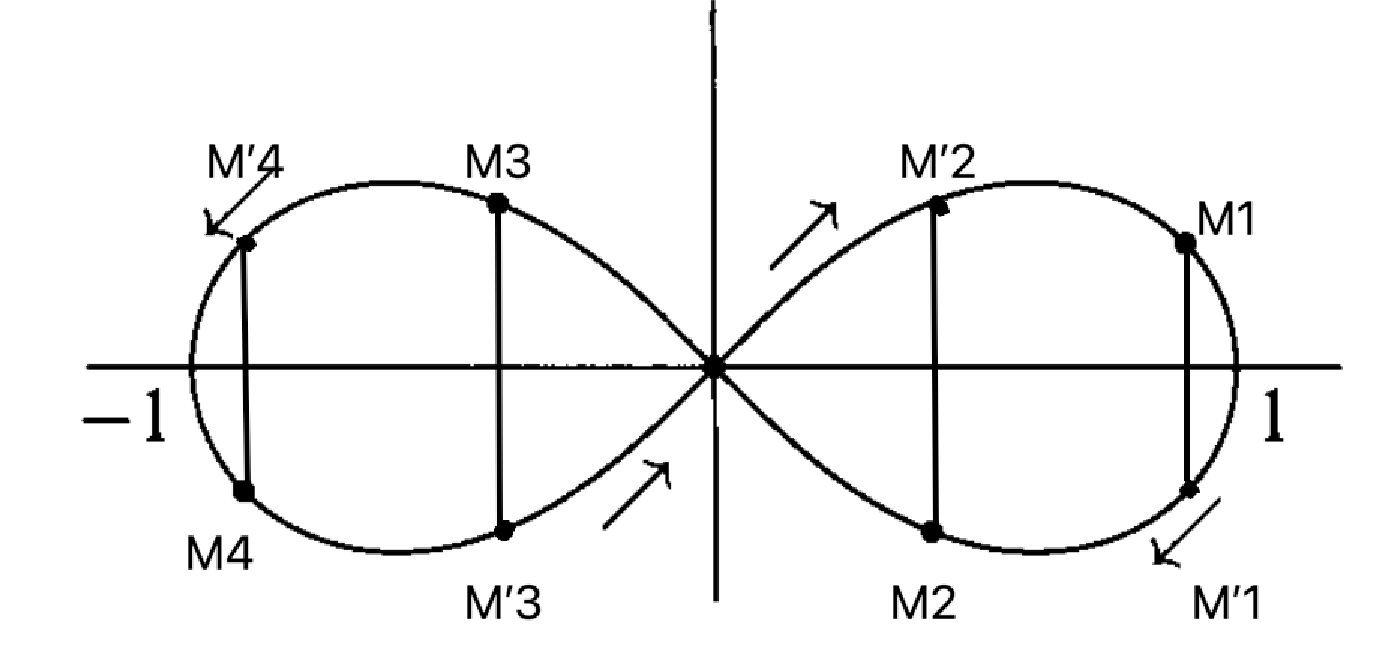
\includegraphics [width=8cm,height=4cm] {lemniscate.png}
\end{center}
\end{figure}
\end{proof}

\paragraph{Ex. 15.1.7}{\it Recall that in Greek geometry, the ellipse is defined to be the locus of all points whose {\bf sum} of distances to two given points is constant. Suppose instead we consider the locus of all points whose {\bf product} of distances to two given points is constant. Show that this leads to (15.7) when the given points are $(a,0),(-a,0)$ and the constant is $b^4$(*).
}

(*) Read $b^2$.

\begin{proof}
Let $\Gamma$ the locus of all points whose product of distances to two points $(a,0),(-a,0)$ is the constant $b^2$. Then
\begin{align*}
M(x,y) \in \Gamma & \iff \sqrt{(x-a)^2 + y^2}   \sqrt{(x+a)^2 + y^2}  = b^2\\
&\iff ((x-a)^2 + y^2)((x-a)^2 + y^2) = b^4.
\end{align*}
We obtain the formula of the ovals of Cassini.
\end{proof}


\subsection{THE LEMNISCATIC FUNCTION}
\paragraph{Ex. 15.2.1}{\it Give a careful proof of (15.9) using the hints given in the text.
}

\begin{proof}
By section 15.2, we know that $\varphi$ is $2\varpi$ periodic,
$$\varphi(s + 2\varpi) = \varphi(s),\qquad (s \in \R).$$
Moreover, for $-1 \leq r \leq 1$, and $\frac{-\varpi}{2} \leq s \leq \frac{\varpi}{2}$,
$$r = \varphi(s) \iff s = \int_0^r \frac{1}{\sqrt{1-t^4}} \D t.$$

Write $r' = \varphi(-s)\in [-1,1]$. Then for every $s \in [-\frac{\varpi}{2} ,\frac{\varpi}{2} ]$,
\begin{align*}
r' = \varphi(-s) & \iff -s = \int_0^{r'} \frac{1}{\sqrt{1-t^4}} \D t\\
&\iff -s = -\int _0^{-r'} \frac{1}{\sqrt{1-\tau^4}} \D \tau\qquad (\tau = -t)\\
&\iff s = \int _0^{-r'} \frac{1}{\sqrt{1-\tau^4}} \D \tau\\
&\iff -r' = \varphi(s)
\end{align*}
This proves that
\begin{align}
\varphi(-s) = - \varphi(s) \qquad \left (-\frac{\varpi}{2} \leq s \leq \frac{\varpi}{2} \right).
\end{align}

Write $M(s)$ the point on the lemniscate with signed arc length $s$. Consider $M' = M(s')$ the symmetric point of $M(s)$ about the origin. Since the lemniscate is symmetric about the origin, 
Consider first the case where $0 \leq s \leq \varpi$, then the signed arc length is the positive arc length. Let $M(s)$ the point on the lemniscate with arc length $s$. Then the symmetric point $M(s')$ about the $x$-axis is such that $r' = OM(s') = OM(s) = r$, thus, by definition of $\varphi$, $\varphi(s) = \varphi(s')$. The total arc length from $O = M(0)$ to $O = M(\varpi)$ in the first loop is $\varpi$, and the symmetry of the lemniscate about the $x$-axis implies that the arc length $\varpi - s$ between $M(s)$ and $O = M(\varpi)$ is equal to the arc length $s'$ between $O = M(0)$ and $M(s')$, thus
$s' = \varpi - s$. This proves
\begin{align}
\varphi(\varpi -s) = \varphi(s)\qquad (0 \leq s \leq \varpi).
\end{align} 

Now, if $\frac{\varpi}{2} \leq s \leq \varpi$, then $0\leq \varpi-s \leq \frac{\varpi}{2}$, thus, using (1), (2), (3)
$$
\left\{
\begin{array}{ll}
\varphi(s) &= \varphi(\varpi - s) = -\varphi(s- \varpi) = -\varphi(s + \varpi),\\
\varphi(-s) &= \varphi(\varpi- (-s)) =\varphi(s + \varpi).
\end{array}
\right.
$$
Therefore $\varphi(-s) = - \varphi(s)$ if $\frac{\varpi}{2} \leq s \leq \varpi$. Now, if we suppose $-\varpi \leq s \leq -\frac{\varpi}{2}$, then $\frac{\varpi}{2} \leq -s \leq \varpi$, so we can apply the last equality to $-s$: $\varphi(s) = \varphi(-(-s))= - \varphi(-s)$. This proves
\begin{align}
\varphi(-s) = \varphi(s) \qquad (-\varpi \leq s \leq \varpi).
\end{align}
Using the periodicity, if $s \in \R$, the is some $n \in \Z$ and $s' \in [-\varpi,\varpi[$ such that $s = 2n\varpi + s'$. Then 
$$\varphi(-s) = \varphi(-s - 2n\varpi) = \varphi(-s') = - \varphi(s') = -\varphi(s-2n\varphi) = - \varphi(s).$$
 We have proved
$$\varphi(-s) = \varphi(s) \qquad (s \in \R).$$
We can now complete (2) to $-\varpi \leq s \leq 0$. Then $0 \leq -s \leq \varpi$, and by (2) applied to $-s$, $\varphi(s + \varpi) = \varphi(-s) = -\varphi(s)$, thus
$$\varphi(\varpi -s) =  - \varphi(s - \varpi) = - \varphi(s+ \varpi) = \varphi(s)$$.

We have proved, for all $s \in \R$,
\begin{align*}
&\varphi(-s) = -\varphi(s)\\
&\varphi(\varpi - s) = \varphi(s).
\end{align*}
\end{proof}

\paragraph{Ex. 15.2.2}{\it Supply the details needed to complete the proof of Proposition 15.2.1.
}

\begin{proof}
The proof of Proposition 15.2.1 shows that
$$\varphi'(s)  = \sqrt{1 - \varphi^4(s)},\qquad 0 \leq s \leq \frac{\varpi}{2}.$$
By Exercise 3, parts (a) and (b), $\varphi'$ is even and has period $2 \varpi$, and by part (c),
$$\varphi'(\varpi - s) = - \varphi'(s), \qquad s \in \R.$$

Therefore, if $-\frac{\varpi}{2} \leq s \leq 0$, then
$$\varphi'(s) = - \varphi'(-s) =  -\sqrt{1 - \varphi^4(-s)} = - \sqrt{1 - \varphi^4(s)}.$$
Now, if $\frac{\varpi}{2} \leq s \leq \varpi$, then $0 \leq \varpi -s \leq \frac{\varpi}{2}$, thus 
$$\varphi'(s) = -\varphi'(\varpi - s) = -\sqrt{1 - \varphi^4(\varpi - s)} = - \sqrt{1 - \varphi^4(s)}.$$
If $-\varpi \leq s \leq -\frac{\varpi}{2}$, then $\frac{\varpi}{2} \leq -s  \leq \varpi$. Using the above equality, we obtain
$$\varphi'(s) = - \varphi(-s) = -  \sqrt{1 - \varphi^4(-s)} = - \sqrt{1 - \varphi^4(s)}.$$
We have proved
$$\varphi'^2(s) = 1 - \varphi^4(s), \qquad -\varpi \leq s \leq \varpi. $$
Now if $s$ is any real number, there is some $n\in \Z$ and $s' \in [-\varpi, \varpi[$ such that $s = 2n \varpi + s'$. Since $2\varpi$ is a period of $\varphi$ and $\varphi'$,
$$\varphi'^2(s) = \varphi'^2(s') = 1 -\varphi^4(s') = 1 - \varphi^4(s).$$
This complete the proof of Proposition 15.2.1.
\end{proof}

\paragraph{Ex. 15.2.3}{\it Here are some useful properties of $\varphi'$.
\be
\item[(a)] $\varphi$ has period $2\varpi$. Explain why this implies that the same is true for $\varphi'$.
\item[(b)] $\varphi$ is an odd function by (15.9). Explain why this implies that $\varphi'$ is even.
\item[(c)] Use (15.9) to prove that $\varphi'(\varpi -s) =  - \varphi'(s)$.
\item[(d)] Use Proposition 15.2.1 to prove that $\varphi''(s) = -2 \varphi^3(s)$.
\ee
}

\begin{proof}
\item[(a)] For all $s \in \R$, $\varphi(s +2 \varpi) = \varphi(s)$. By differentiation, and the chain rule,  we obtain
$$\varphi'(s + 2 \varphi)(s)= \varphi(s).$$
$\varphi'$ has period $2 \varpi$.
\item[(b)] Since $\varphi(-s) = - \varphi(s)$ for all $s \in \R$, the chain rule gives
$$- \varphi'(-s) = - \varphi'(s),$$
thus $\varphi'$ is even.
\item[(c)] By (15.9), $\varphi(\varpi - s) = \varphi(s)$ for all $s \in \R$. Then the chain rule gives $-\varphi'(\varpi -s) = \varphi'(s)$, thus
$$\varphi'(\varpi -s) = -\varphi'(s),\qquad s \in \R.$$
\item[(d)] By differentiation of $\varphi'^2(s) = 1 - \varphi^4(s)\ (s \in \R)$, we obtain
$$2 \varphi'(s) \varphi''(s) = -4 \varphi^3(s) \varphi'(s).$$
If $s \ne \frac{\varpi}{2} + n \varpi, n \in \Z$, then $\varphi'(s) \ne 0$, so that
$$\varphi''(s) = -2 \varphi^3(s),\qquad s \ne \frac{\varpi}{2} + n \varpi, n \in \Z.$$
If $s=\frac{\varpi}{2} + n \varpi $ for some integer $n \in \Z$, since $\varphi$ is infinitely differentiable, $\varphi''$ is continuous, therefore
$$\varphi''(s) = \lim_{t \to s, t\ne s} \varphi''(t) = \lim_{t \to s, t \ne s} (-2 \varphi^3(t)) = -2 \varphi^3(s).$$
Therefore
$$\varphi''(s) = -2 \varphi^3(s),\qquad s \in \R.$$
\end{proof}

\paragraph{Ex. 15.2.4}{\it Suppose that we define $\sin(x)$ by $y = \sin(x) \iff x = \int_0^y(1-t^2)^{-1/2} \D t$. Then define $\cos (x)$ to be $sin'(x)$. Use the method of Proposition 15.2.1 to prove the standard trigonometric identity $\cos^2(x) = 1 - \sin^2(x)$.
}

\begin{proof}
We obtain the analog of (15.9) as in Exercise 1: for all $x \in \R$,
\begin{align*}
\sin(-x) = - \sin(x),\\
\sin(\pi-x) = \sin(x).
\end{align*}

Now we use the definition of $\sin$: for all $y\in [-1,1]$, for all $x \in [-\frac{\pi}{2}, \frac{\pi}{2}]$,
$$y = \sin(x) \iff x = \int_0^y(1-t^2)^{-1/2} \D t,$$
where $\int_0^1(1-t^2)^{-1/2} \D t$ and $ \int_0^{-1}(1-t^2)^{-1/2} \D t$ converge.

If $x \in [0 , \frac{\pi}{2}[$, differentiating each side of
$$s = \int_0^{\sin(x)} \frac{1}{\sqrt{1-t^2}} \D t,$$
we obtain
$$1 = \frac{1}{\sqrt{1 - \sin^2(x)}} \sin'(x).$$
If $x = \frac{\pi}{2}$, then $\sin(x) = 1, \sin'(x) = 0$, thus $\sin'^2(x) = 1 - \sin^2(x)$.
Therefore
$$\cos(x) = \sin'(x) = \sqrt{1 - \sin^2(x)},\qquad 0 \leq x \leq \frac{\pi}{2}.$$
We extend the equality $\sin^2(x) + \cos^2(x) = 1$ to all $x \in \R$ as in Exercise 2.
\end{proof}

\paragraph{Ex. 15.2.5}{\it Here is Abel's proof of the addition law for $\varphi$.
\be
\item[(a)]
Let $g(x,y)$ be differentiable on $\R^2$, and set $h(u,v) = g\left(\frac{1}{2}(u+v), \frac{1}{2}(u-v)\right)$. Use the chain Rule to prove that
$$\frac{\partial h}{\partial v}(u,v) = \frac{1}{2}\frac{\partial g}{\partial x}\left(\frac{1}{2}(u+v), \frac{1}{2}(u-v)\right)-\frac{1}{2}\frac{\partial g}{\partial y}\left(\frac{1}{2}(u+v), \frac{1}{2}(u-v).\right)$$
\item[(b)] Use part (a) to show that $g(x,y) = g(x+y, 0)$ on, $\R^2$ if and only if $\frac{\partial g}{\partial x} = \frac{\partial g}{\partial y}$ on $\R^2$.
\item[(c)] Prove the addition law for $\varphi$ by applying part (b) to
$$g(x,y) = \frac{\varphi(x) \varphi'(y) + \varphi(y) \varphi'(x)}{1 + \varphi^2(x) \varphi^2(y)}.$$
Part (d) of Exercise 3 will be useful.
\ee
}

\begin{proof} 
\item[(a)] To apply the Chain Rule, we suppose that $g$ is continuously differentiable ($g \in C_1(\R^2)$). Write $x,y : \R^2 \to \R^2$ the two maps defined by
$$x(u,v) = \frac{1}{2}(u+v),\qquad y(u,v) = \frac{1}{2}(u-v),$$
Then 
$$\frac{\partial x}{\partial v}(u,v) = \frac{1}{2},\qquad \frac{\partial y}{\partial v}(u,v) = -\frac{1}{2},$$
and
$$h(u,v) = g(x(u,v),y(u,v)),\qquad (u,v)\in \R^2.$$
The Chain Rule gives
\begin{align*}
\frac{\partial h}{\partial v}(u,v)&=\frac{\partial g}{\partial x}\left(x(u,v),y(u,v)\right)\frac{\partial x}{\partial v}(u,v)+\frac{\partial g}{\partial y}\left(x(u,v),y(u,v)\right)\frac{\partial y}{\partial v}(u,v)\\
&=\frac{1}{2}\frac{\partial g}{\partial x}\left(\frac{1}{2}(u+v), \frac{1}{2}(u-v)\right)-\frac{1}{2}\frac{\partial g}{\partial y}\left(\frac{1}{2}(u+v), \frac{1}{2}(u-v)\right)
\end{align*}

\item[(b)] 

Suppose that $g(x+y,0) = g(x,y)$ for all $x,y \in \R$. Write $f(x) = g(x,0)$. Then $f$ is continuously differentiable, and $g(x,y) = f(x+y)$. By the Chain Rule, for all $(x,y) \in \R^2$,
$$
\frac{\partial g}{\partial x}(x,y) = f'(x+y) = \frac{\partial g}{\partial y}(x,y),
$$
therefore $\frac{\partial g}{\partial x} = \frac{\partial g}{\partial y}$ on $\R^2$.

\qquad

Conversely, suppose that $\frac{\partial g}{\partial x} = \frac{\partial g}{\partial y}$ on $\R^2$. Then, for all $(u,v) \in \R^2$,
$$\frac{\partial h}{\partial v}(u,v) = \frac{1}{2}\frac{\partial g}{\partial x}\left(\frac{1}{2}(u+v), \frac{1}{2}(u-v)\right)-\frac{1}{2}\frac{\partial g}{\partial y}\left(\frac{1}{2}(u+v), \frac{1}{2}(u-v) \right)= 0.$$
This means that for every fixed $u_0 \in \R$, the map $v \mapsto h(u_0,v)$ has a null derivative, thus is constant: $h(u_0,v) = h(u_0,0)$ for all $v \in \R$. Since this is true for every $u_0$, we obtain 
$$h(u,v) = h(u,0),\qquad \text{for all } u,v \in \R.$$
Write $f(u) = h(u,0)$ for all $u\in \R$. Then $f$ is continuously differentiable, and for all $u,v \in \R$, $h(u,v) = f(u)$ depends only of $u$.

By definition of $h$, this means that, for all $u,v \in \R$,
$$g\left(\frac{1}{2}(u+v), \frac{1}{2}(u-v)\right) = f(u).$$
Taking $v = u$ in $g\left(\frac{1}{2}(u+v), \frac{1}{2}(u-v)\right) = h(u,v) = h(u,0)$, we obtain $g(u,0) = h(u,u) = h(u,0)$, therefore
$$g(u,0) = h(u,u) = h(u,0) = h(u,v) = g\left(\frac{1}{2}(u+v), \frac{1}{2}(u-v)\right),$$
thus
$$g(u,0) = g\left(\frac{1}{2}(u+v), \frac{1}{2}(u-v)\right),\qquad u,v \in \R.$$
If $(x,y)$ is any pair in $\R^2$, there exists a unique pair $(u,v) \in \R^2$ such that $x = \frac{1}{2}(u+v), y = \frac{1}{2}(u-v)$, given by $u = x + y, v = x-y$. Therefore, the preceding equality implies that 
$$g(x+y,0) = g(x,y) ,\qquad x,y \in \R.$$ 

\item[(c)] Define $g : \R^2 \to \R$ by
$$g(x,y) = \frac{\varphi(x) \varphi'(y) + \varphi(y) \varphi'(x)}{1 + \varphi^2(x) \varphi^2(y)}.$$
The partial derivative of this quotient relative to the variable $x$ gives, using $\varphi''(x) = -2 \varphi^3(x)$ (see Exercise 3, part (d)), and $\varphi'(x)^2 = 1 -\varphi^4(x)$
\begin{align*}
&\left(1 + \varphi^2(x)\varphi^2(y)\right)^2 \frac{\partial g}{\partial x} (x,y) \\
&= \left(\varphi'(x) \varphi'(y) + \varphi(y) \varphi''(x)\right)\left(1+ \varphi^2(x)\varphi^2(y)\right) - 2 \varphi(x) \varphi'(x) \varphi^2(y) \left(\varphi(x) \varphi'(y)+ \varphi(y)\varphi'(x)\right)\\
&= \left(\varphi'(x) \varphi'(y) -2 \varphi(y)\varphi^3(x)\right)\left(1+ \varphi^2(x)\varphi^2(y)\right) - 2 \varphi(x) \varphi'(x) \varphi^2(y) \left(\varphi(x) \varphi'(y)+ \varphi(y)\varphi'(x)\right)\\
&=\varphi'(x) \varphi'(y) + \varphi'(x) \varphi'(y) \varphi^2(x) \varphi^2(y) - 2 \varphi(y) \varphi^3(x) - 2 \varphi^3(y)\varphi^5(x)\\
&  \qquad - 2 \varphi^2(x) \varphi^2(y) \varphi'(x)\varphi'(y) - 2 \varphi(x) \varphi^3(y) \varphi'(x)^2\\
&=\varphi'(x) \varphi'(y) + \varphi'(x) \varphi'(y) \varphi^2(x) \varphi^2(y) - 2 \varphi(y) \varphi^3(x) - 2 \varphi^3(y)\varphi^5(x)\\
&  \qquad - 2 \varphi^2(x) \varphi^2(y) \varphi'(x)\varphi'(y) - 2 \varphi(x) \varphi^3(y) (1 - \varphi^4(x))\\
&=\varphi'(x) \varphi'(y) + \varphi'(x) \varphi'(y) \varphi^2(x) \varphi^2(y) - 2 \varphi(y) \varphi^3(x) -2\varphi(x) \varphi^3(y)\\
&  \qquad - 2 \varphi^2(x) \varphi^2(y) \varphi'(x)\varphi'(y).
\end{align*}
This last expression is symmetric relatively to $x,y$, and also the denominator $(1 + \varphi^2(x)\varphi^2(y))^2$.  Since $g(x,y) = g(y,x) =  \frac{\varphi(y) \varphi'(x) + \varphi(x) \varphi'(y)}{1 + \varphi^2(y) \varphi^2(x)}$, this proves that 
\begin{align*}
&\left(1 + \varphi^2(y)\varphi^2(x)\right) \frac{\partial g}{\partial y} (x,y)\\
&=\varphi'(y) \varphi'(x) + \varphi'(y) \varphi'(x) \varphi^2(y) \varphi^2(x) - 2 \varphi(x) \varphi^3(y) -2\varphi(y) \varphi^3(x)- 2 \varphi^2(y) \varphi^2(x) \varphi'(y)\varphi'(x)\\
&= \left(1 + \varphi^2(x)\varphi^2(y)\right) \frac{\partial g}{\partial x} (x,y),
\end{align*}
where $1 + \varphi^2(y)\varphi^2(x)>0$.
Therefore $\frac{\partial g}{\partial x} = \frac{\partial g}{\partial y}$ on $\R^2$. 

By part (b), $g(x,y) =g(x+y,0)$. Using $\varphi(0) = 0$, and $\varphi'(0) = \sqrt{1 - \varphi^4(0)} = 1$, 
\begin{align*}
g(x,y) &=g(x+y,0)\\
&= \varphi'(0) \varphi(x+y)\\
&= \varphi(x+y).
\end{align*}
We have proved the addition law for $\varphi$:
$$\varphi(x+y) = \frac{\varphi(x) \varphi'(y) + \varphi(y) \varphi'(x)}{1 + \varphi^2(x) \varphi^2(y)}, \qquad x,y \in \R.$$
\end{proof}

\paragraph{Ex. 15.2.6}{\it Show that the subtraction law
$$\varphi(x-y) = \frac{\varphi(x) \varphi'(y) - \varphi(y) \varphi'(x)}{1 + \varphi^2(x) \varphi^2(y)}.
$$
follows from the addition law together with (15.9) and Exercise 3.
}

\begin{proof} Starting from the Addition Law for $\varphi$
$$\varphi(x+y) = \frac{\varphi(x) \varphi'(y) + \varphi(y) \varphi'(x)}{1 + \varphi^2(x) \varphi^2(y)}, \qquad x,y \in \R,$$
we obtain for all $x,y \in \R$, substituting $-y$ to $y$,
\begin{align*}
&\varphi(x-y) = \frac{\varphi(x) \varphi'(-y) + \varphi(-y) \varphi'(x)}{1 + \varphi^2(x) \varphi^2(-y)}.
\end{align*}
Since $\varphi$ is odd, and $\varphi'$ even (see 15.9 and Exercise 3), we obtain
$$\varphi(x-y) = \frac{\varphi(x) \varphi'(y) - \varphi(y) \varphi'(x)}{1 + \varphi^2(x) \varphi^2(y)}.
$$
\end{proof}

\paragraph{Ex. 15.2.7}{\it The proof of Theorem 15.2.5 uses induction on $n$.
\be
\item[(a)] Assume that $n$ is even. In (15.18), we gave a formula for $Q_{n+1}(u)$ in terms of $Q_n(u)$ and $Q_{n-1}(u)$. Derive the corresponding formula for $P_{n+1}(u)$.
\item[(b)] Suppose that polynomials $P_n(u),Q_n(u)$ satisfy all of the conditions of the theorem except for the requirement that they be relatively prime. Since $\Z[u]$ is a $UFD$, we can write $P_n(u) = C_n \tilde{P}_n(u), Q_n(u) = C_n(u) \tilde{Q}_n(u)$, where $C_n(u), \tilde P_n(u),\tilde Q_n(u) \in \Z[u]$ and $\tilde P_n(u), \tilde Q_n(u)$ are relatively prime. Prove that we can assume that $\tilde Q_n(0) = 1$ and that $\tilde P_n(u), \tilde Q_n(u)$ satisfy all conditions of Theorem 15.2.5.
\item[(c)] Complete the inductive step of the proof when $n$ is odd.
\ee
}

\begin{proof} 
\item[(a,c)] We will prove the theorem by induction on $n$. The theorem holds for $n=1,n=2$  with $P_1(u) =  Q_1(u) = 1$, and $P_2(u) = 2,Q_2(u) = 1+u$ (misprint in Cox p. 477).
Now assume that it holds for $n-1$ and $n$.

$\bullet$
If $n$ is even,
\begin{align*}
& \varphi((n-1)x) = \varphi(x)\frac{P_{n-1}\left(\varphi^4(x)\right)}{Q_{n-1}\left(\varphi^4(x)\right)}, \\
 &\varphi(nx) = \varphi(x)\frac{P_{n}\left(\varphi^4(x)\right)}{Q_{n}\left(\varphi^4(x)\right)} \varphi'(x).
  \end{align*}
 Using (15.13), we obtain
\begin{align*}
\varphi\left((n+1)x\right) &= - \varphi\left( (n-1)x) \right) + \frac{2 \varphi(nx) \varphi'(x)}{1+\varphi^2(nx) \varphi^2(x)}\\
&=- \varphi(x) \frac{P_{n-1}\left(\varphi^4(x)\right)}{Q_{n-1}\left(\varphi^4(x)\right)} + \frac{2 \left(\varphi(x)\frac{P_{n}\left(\varphi^4(x)\right)}{Q_{n}\left(\varphi^4(x)\right)} \varphi'(x) \right) \varphi'(x)}{1+\left(\varphi(x)\frac{P_{n}\left(\varphi^4(x)\right)}{Q_{n}\left(\varphi^4(x)\right)} \varphi'(x) \right)^2 \varphi^2(x)}.\\
\end{align*}
To simplify, we write $a = \varphi(x), p_n = P_n(\varphi^4(x)), q_n = Q_n(\varphi^4(x))$. 

Then, using $\varphi'(x)^2 = 1 - \varphi^4(x)$,
\begin{align*}
\varphi\left((n+1)x\right) &= a \left[ -\frac{p_{n-1}}{q_{n-1}} + \frac{2 (1-a^4)\frac{p_n}{q_n} }{1 + a^4(1-a^4) \frac{p_n^2}{q_n^2}} \right] \\
&=a \left[  -\frac{p_{n-1}}{q_{n-1}} + \frac{2(1-a^4)p_nq_n}{q_n^2+a^4(1-a^4)p_n^2}\right] \\
&=a \frac {-p_{n-1}(q_n^2 + a^4(1-a^4) p_n^2) + 2(1-a^4) p_nq_nq_{n-1}}{q_{n-1}(q_n^2 + a^4(1-a^4)p_n^2)},
\end{align*}
that is
$$\varphi\left((n+1)x\right) = \varphi(x) \frac{P_{n+1}(\varphi^4(x))}{Q_{n+1}(\varphi^4(x))},$$
where
\begin{align*}
P_{n+1}(u) &= -P_{n-1}(u) (Q_n^2(u) + u(1-u) P_n^2(u)) + 2(1-u) P_n(u)Q_n(u) Q_{n-1}(u),\\
Q_{n+1}(u) &=Q_{n-1}(u)(Q_n^2(u) + u(1-u) P_n^2(u)).
\end{align*}
Verification : with $n = 2$, we obtain $P_3(u) = 3 - 6u - u^2, Q_3(u) = 1 + 6u - 3u^2$, which gives the tripling formula (15.17).

\qquad

$\bullet$ If $n$ is odd,
\begin{align*}
& \varphi((n-1)x) = \varphi(x)\frac{P_{n-1}\left(\varphi^4(x)\right)}{Q_{n-1}\left(\varphi^4(x)\right)} \varphi'(x), \\
 &\varphi(nx) = \varphi(x)\frac{P_{n}\left(\varphi^4(x)\right)}{Q_{n}\left(\varphi^4(x)\right)} .
  \end{align*}
  Then(15.13) gives
  \begin{align*}
\varphi\left((n+1)x\right) &= - \varphi\left( (n-1)x) \right) + \frac{2 \varphi(nx) \varphi'(x)}{1+\varphi^2(nx) \varphi^2(x)}\\
&=- \varphi(x) \frac{P_{n-1}\left(\varphi^4(x)\right)}{Q_{n-1}\left(\varphi^4(x)\right)}  \varphi'(x)+ \frac{2 \left(\varphi(x)\frac{P_{n}\left(\varphi^4(x)\right)}{Q_{n}\left(\varphi^4(x)\right)}  \right) \varphi'(x)}{1+\left(\varphi(x)\frac{P_{n}\left(\varphi^4(x)\right)}{Q_{n}\left(\varphi^4(x)\right)}  \right)^2 \varphi^2(x)}\\
&=\varphi(x) \left[ -  \frac{P_{n-1}\left(\varphi^4(x)\right)}{Q_{n-1}\left(\varphi^4(x)\right)} + \frac{2 \left(\frac{P_{n}\left(\varphi^4(x)\right)}{Q_{n}\left(\varphi^4(x)\right)}  \right) }{1+\left(\varphi(x)\frac{P_{n}\left(\varphi^4(x)\right)}{Q_{n}\left(\varphi^4(x)\right)}  \right)^2 \varphi^2(x)}\right] \varphi'(x)
\end{align*}
With the same notations as in the even case, and with $a' = \varphi'(x)$, 
\begin{align*}
\varphi\left((n+1)x\right)&= a \left[ -\frac{p_{n-1}}{q_{n-1}} + \frac{2 \frac{p_n}{q_n}}{1 + a^4 \frac{p_n^2}{q_n^2}}\right] a'\\
&= a \left[ -\frac{p_{n-1}}{q_{n-1}}  +\frac{ 2 p_n q_n}{q_n^2 + a^4 p_n^2}\right] a' \\
&=a\left[ \frac{-p_{n-1} (q_n^2 + a^4 p_n^2) + 2 p_nq_nq_{n-1}} {q_{n-1}(q_n^2 + a^4 p_n^2)}\right] a'
\end{align*}
that is
$$\varphi\left((n+1)x\right) = \varphi(x) \frac{P_{n+1}(\varphi^4(x))}{Q_{n+1}(\varphi^4(x))}\varphi'(x),$$
where
\begin{align*}
P_{n+1}(u) &= -P_{n-1}(u) (Q_n^2(u) + u P_n^2(u)) + 2 P_n(u)Q_n(u) Q_{n-1}(u),\\
Q_{n+1}(u) &=Q_{n-1}(u)(Q_n^2(u) + u P_n^2(u)).
\end{align*}
The induction is done, and the induction formulas concerning $P_{n}, Q_{n}$ are
$$\begin{array}{ll}
&\text {for } n \text { even},\\
P_{n+1}(u) &= -P_{n-1}(u) (Q_n^2(u) + u(1-u) P_n^2(u)) + 2(1-u) P_n(u)Q_n(u) Q_{n-1}(u),\\
Q_{n+1}(u) &=Q_{n-1}(u)(Q_n^2(u) + u(1-u) P_n^2(u)),\\
&\text {for } n \text { odd},\\
P_{n+1}(u) &= -P_{n-1}(u) (Q_n^2(u) + u P_n^2(u)) + 2 P_n(u)Q_n(u) Q_{n-1}(u),\\
Q_{n+1}(u) &=Q_{n-1}(u)(Q_n^2(u) + u P_n^2(u)).
\end{array}
$$
Note that we can take $P_0 = 0, Q_1 = 1$ ( and $P_1 = 1, Q_1 = 1$).

\bigskip

We give a Sage function to compute $P_n,Q_n$:
\begin{verbatim}
R.<u> = ZZ[]

def divisionPolynomial(n):
    P0, Q0 = 0, 1
    P1, Q1 = 1, 1
    for i in range(n):
        if i % 2 != 0:
            S = Q1^2 + u * (1-u) *P1^2
            P2 = -P0 * S + 2 * (1-u) * P1 * Q1 * Q0
            Q2 = Q0  * S
        else:
            S = Q1^2 + u * P1^2
            P2 = -P0 * S + 2 * P1 * Q1 * Q0
            Q2 = Q0  * S
        D = gcd(P2,Q2)
        (P2, Q2) = (P2/D, Q2/D)
        (P0, Q0) = (P1, Q1)
        (P1, Q1) = (P2, Q2)
    return (P0,Q0)
    
P5, Q5 = divisionPolynomial(5); P5,Q5
\end{verbatim}
$$u^{6} + 50u^{5} - 125u^{4} + 300u^{3} - 105u^{2} - 62u + 5,  5u^{6} - 62u^{5} - 105u^{4} + 300u^{3} - 125u^{2} + 50u + 1$$
\begin{verbatim}
P5.factor(), Q5.factor()
\end{verbatim}
$$(u^{2} - 2u + 5) \cdot (u^{4} + 52u^{3} - 26u^{2} - 12u + 1), (5u^{2} - 2u + 1) \cdot (u^{4} - 12u^{3} - 26u^{2} + 52u + 1)$$
\item[(b)] We can write $P_n(u) = C_n \tilde{P}_n(u), Q_n(u) = C_n(u) \tilde{Q}_n(u)$, where $C_n(u), \tilde P_n(u),\tilde Q_n(u) \in \Z[u]$ and $\tilde P_n(u), \tilde Q_n(u)$ are relatively prime.

Since $Q_n(0) = 1$, then $C_n(0) \tilde{Q}_n(0) = 1$, where $C_n(0), \tilde{Q}_n(0)$ are integers, thus $\tilde{Q}_n(0) = \pm 1$.

If $\tilde{Q}_n(0) = 1$, we are done, and if $\tilde{Q}_n(0) = -1$ We replace $\tilde{P}_n, \tilde{Q}_n$ by $-\tilde{P}_n, - \tilde{Q}_n$, which satisfy all conditions of Theorem 15.2.5.
\end{proof}

\paragraph{Ex. 15.2.8}{\it Let $n$ be even, and let $P_n(u)$ be the polynomial from Theorem 15.2.5. Complete the proof of Corollary 15.2.6 by showing that the polar distances of the $n$-division points of the lemniscate are roots of $uP_n(u^4)(1-u^2)$.
}

\begin{proof} 
The polar distances of the $n$-division points are
$$u_m = \varphi\left( m \frac{2 \varpi}{n}\right),\qquad m=0,1,\ldots,n-1.$$
If $n$ is even, then 
$$\varphi(nx) = \varphi(x)\frac{P_{n}\left(\varphi^4(x)\right)}{Q_{n}\left(\varphi^4(x)\right)} \varphi'(x).$$
With $x = \frac{2 \varpi}{n}$, we obtain
$$0 = \varphi(m \cdot 2 \varpi) = \varphi\left(n\cdot  m \frac{2 \varpi}{n}\right) = \varphi\left( m \frac{2 \varpi}{n}\right)\frac{P_n\left(\varphi^4\left( m \frac{2 \varpi}{n}\right)\right)}{Q_n\left(\varphi^4\left( m \frac{2 \varpi}{n}\right)\right)}\varphi'\left(m \frac{2 \varpi}{n}\right),$$
where, by Exercise 9, the denominator $Q_n\left(\varphi^4\left( m \frac{2 \varpi}{n}\right)\right)$ is non vanishing.

Since $\varphi'\left(m \frac{2 \varpi}{n}\right) = \pm\sqrt{1 - \varphi^4\left(m \frac{2 \varpi}{n}\right)}$, we obtain
$$0 = u_m P_n(u_m^4) \sqrt{1 - u_m^4}.$$
$\sqrt{1 - u_m^4} = \sqrt{1 - u_m^2} \sqrt{1+u_m^2}$, where $1+ u_m^2 \ne 0$, thus $\sqrt{1 -u_m^4} = 0 \iff 1 - u_m^2 = 0$. Therefore $u_m= \varphi\left( m \frac{2 \varpi}{n}\right)$ is a root of 
$$u P_n(u^4)(1-u^2).$$
\end{proof}

\paragraph{Ex. 15.2.9}{\it This exercise is concerned with the proof of Corollary 15.2.7.
\be
\item[(a)] Suppose that $P(u), Q(u) \in \Z[u]$ are relatively prime and $Q(0) = 1$. Prove that $uP(u^4)$ and $Q(u^4)$ have no common roots in any extension of $\Q$.
\item[(b)] Fix $x$ in $\R$ and $m>0$ in $\Z$, and let $P_m(u),Q_m(u) \in \Z[u]$ be as in Theorem 15.2.5. Thus $\varphi(mx) Q_m(\varphi^4(x)) = \varphi(x) P_m(\varphi^4(x))$. Prove that $Q_m(\varphi^4(x)) \ne 0$ when $\varphi(x)\ne 0$.
\item[(c)] Show that $\varphi\left(\frac{2 \varpi}{n}\right) \ne 0$ when $n>2$ is in $\Z$ and conclude that $Q_m\left(\varphi^4\left(\frac{2 \varpi}{n}\right)\right) \ne 0$.
\ee
}

\begin{proof} 
\item[(a)]
Since $P(u),Q(u)$ are relatively prime in $\Q[u]$, there are some polynomials $A,B \in \Q[u]$ such that $A(u)P(u) + B(u) Q(u) = 1$, thus the substitution $u \to u^4$ gives $A(u^4) P(u^4) + B(u^4)Q(u^4) = 1$. Reasoning by contradiction, suppose that $uP(u^4)$ and $Q(u^4)$ have a common root $\alpha$ in some extension of $\Q$. Since $Q(0) = 1$, $\alpha \ne 0$, thus $P(\alpha^4) = 0$.  Then $P(\alpha^4)= Q(\alpha^4) = 0$ implies $1 = A(\alpha^4) P(\alpha^4) + B(\alpha^4)Q(\alpha^4) = 0$: this is a contradiction. 

So $uP(u^4)$ and $Q(u^4)$ have no common roots in any extension of $\Q$.

\item[(b)] If $m$ is odd, then $\varphi(mx) Q_m(\varphi^4)(x)) = \varphi(x) P_m(\varphi^4(x))$. Reasoning by contradiction, suppose that, for some $x \in \R$, $Q_m(\varphi^4(x)) = 0$. Then $\varphi(x) P_m(\varphi^4(x) = 0$, so that $\alpha = \varphi(x)$ is a common root of $Q_m(u^4)$ and $uP_m(u^4)$. Since $P_m,Q_m$ are relatively prime, and $Q_m(0) = 1$, this is impossible by part (a).

If $m$ is even, then $\varphi(mx) Q_m(\varphi^4(x)) = \varphi(x) P_m(\varphi^4(x)) \varphi'(x)$. Suppose that, for some $x \in \R$, $Q_m(\varphi^4(x)) = 0$. Then $\varphi(x) P_m(\varphi^4(x) ) \varphi'(x)= 0$. If $\varphi'(x) =0$, then $\sqrt{1 - \varphi^4(x)} = 0$, thus $\varphi^4(x) = 1$, and $\varphi(x) = \pm 1$. If $\varphi(x) \not \in \{-1,1\}$, then $\varphi(x) P_m(\varphi(x)) =0$, so that $\alpha = \varphi(x)$ is a common root of $Q_m(u^4)$ and $uP_m(u^4)$, which is impossible by part (a).

We have proved that $Q_m(\varphi^4(x)) \ne 0$ when $\varphi(x)\not \in \{-1,1\}$.

(Misprint in the sentence of part (b) ? If $\varphi(x) = 0$, then $Q_m(\varphi^4(x)) = Q_m(0) = 1 \ne 0$, so there is no need to suppose $\varphi(x) \ne 0$.)
\item[(c)] For all $x \in \R$, $\varphi(x) = 0 $ if and only if $x = k \varpi$ for some $k \in \Z$.

We must verify that $\varphi\left(\frac{2\varpi}{n}\right) \not \in \{-1,1\}$. If $n>2$, then $0<\frac{2\varpi}{n}\ < \varpi$. This proves that $0 < \varphi\left(\frac{2\varpi}{n}\right) <1$, thus $\varphi\left(\frac{2\varpi}{n}\right) \not \in \{-1,0,1\}$.

By our version of part (b), this implies that $$Q_m\left(\varphi^4\left(\frac{2\varpi}{n}\right)\right) \ne 0.$$

Note: If we read the proof of Theorem 15.2.5, it is obvious that the denominators $Q_n(\varphi^4(x))$ never vanish, for all $x \in \R$, because $1 + \varphi^2(nx) \varphi^2(x) \ne 0$.
\end{proof}

\paragraph{Ex. 15.2.10}{\it The polar distances of the $5$-division points of the lemniscate satisfy the equation
$$0 = r_0(r_0^{24} + 50 r_0^{20} - 125 r_0^{16} + 300 r_0^{12} - 105 r_0^8 - 62 r_0^4 + 5).$$
This equation was first derived by Fagnano in 1718.
\be
\item[(a)] Show that the $r_0$ corresponding to the $10$-division points also satisfy this equation.
\item[(b)] Use Maple or Mathematica (or Sage!) to show that this equation factors as
$$0 = r_0(r_0^8 - 2 r_0^4 + 5)(r_0^{16}+52r_0^{12} - 26 r_0^8 - 12 r_0^4 + 1)$$
and that the only positive real solutions are
$$\sqrt[4]{-13 + 6 \sqrt{5} \pm 2 \sqrt{85-38 \sqrt{5}}}.$$
Explain (with a picture) how these solutions relate to the $5$- and $10$-division points.
\ee
}

\begin{proof} 
\item[(a)] Since $5$ is odd, the $5$-division points are roots of $uP_5(u^4)$ by Corollary 15.2.6.
We obtain $P_5$ with the Sage function given in Exercise 7:
$$P_5(u) = u^{6} + 50u^{5} - 125u^{4} + 300u^{3} - 105u^{2} - 62u + 5.$$
Therefore the polar distances $r_0$ of the $5$-divisions points of the lemniscate satisfy the equation
$$0 = r_0(r_0^{24} + 50 r_0^{20} - 125 r_0^{16} + 300 r_0^{12} - 105 r_0^8 - 62 r_0^4 + 5).$$

\bigskip

We have seen in Exercise 6 that the $10$-division points are the $5$-divisions points, together with the symmetric points about the $x$-axis, which have same polar distances. Therefore the polar distance of any $10$-division point is also a polar distance of a $5$-division point, thus verify the given equation (see figure in Exercise 6).

\item[(b)]  We saw in Exercise 7 that $P_5(u)$ factors as
$$P_5(u) = (u^{2} - 2u + 5) (u^{4} + 52u^{3} - 26u^{2} - 12u + 1).$$
Therefore the polar distances of the $5$-division points (and of the $10$-division points) satisfy
$$0 = r_0P_5(r_0^4) =r_0 (r_0^{8} - 2r_0^{4} + 5)  (r_0^{16} + 52r_0^{12} - 26r_0^{8} - 12r_0^4 + 1).$$
$r_0^{8} - 2r_0^{4} + 5 = (r_0^4-1)^2 + 4 >0$ thus $r_0^{8} - 2r_0^{4} + 5$ has no real root.

We obtain the positive roots of $u^{4} + 52u^{3} - 26u^{2} - 12u + 1$ with Sage:
\begin{verbatim}
u = var('u')
P = u^4+52*u^3-26*u^2-12*u+1;
S = P.solve(u)
S
\end{verbatim}
\begin{align*}\
[u = -6 \, \sqrt{5} - \frac{1}{2} \, \sqrt{608 \, \sqrt{5} + 1360} - 13, \\
u = -6 \, \sqrt{5} + \frac{1}{2} \, \sqrt{608 \, \sqrt{5} + 1360}- 13, \\
u = 6 \, \sqrt{5} - \frac{1}{2} \, \sqrt{-608 \, \sqrt{5} + 1360}- 13,\\
 u = 6 \, \sqrt{5} + \frac{1}{2} \, \sqrt{-608 \, \sqrt{5} + 1360}- 13]
\end{align*}
\begin{verbatim}
[e.right().n() for e in S]
\end{verbatim}
$$\left[-52.4909612184115, -0.341854511585989, 0.0733810146911846,0.759434715306293\right]$$
\begin{verbatim}
S[2].right()^(1/4),S[3].right()^(1/4)
\end{verbatim}
$$\left({\left(6 \, \sqrt{5} - \frac{1}{2} \, \sqrt{-608 \, \sqrt{5} +
1360} - 13\right)}^{\frac{1}{4}}, {\left(6 \, \sqrt{5} + \frac{1}{2} \,
\sqrt{-608 \, \sqrt{5} + 1360} - 13\right)}^{\frac{1}{4}}\right)$$

Since $1360 = 1 6 \times 85$, and $608 = 16 \times 38$, we obtain the two positive solutions of the equation
$$\sqrt[4]{-13 + 6 \sqrt{5} \pm 2 \sqrt{85-38 \sqrt{5}}}.$$
Since there are only two $5$-division points $M_1,M_2$ in the right loop of the lemniscate, the 5 division points have polar distances (using $OM_1 > OM_2$)
\begin{align*}
&OM_0   = 0 \\
&OM_1  = OM_4= \left( \sqrt[4]{-13 + 6 \sqrt{5} +2 \sqrt{85-38 \sqrt{5}}} \right),\\
 &OM_2  = OM_3  = \left( \sqrt[4]{-13 + 6 \sqrt{5} - 2 \sqrt{85-38 \sqrt{5}}} \right).\\
 \end{align*}
 (See the figure of Exercise 6). 
 
 By Proposition 15.1.1, all these points are constructible. The $10$-division points have same polar distances, and are also constructible.
\end{proof}

\paragraph{Ex. 15.2.11}{\it Use $\sin(x+y) = \sin x \cos y + \sin y \cos x$ to show that if $\alpha,\beta \in [0,1]$, then
$$\int_0^\alpha \frac{1}{\sqrt{1-t^2}} \D t + \int_0^\beta \frac{1}{\sqrt{1-t^2}} \D t  = \int_0^\gamma \frac{1}{\sqrt{1-t^2}} \D t,$$
where $\gamma$ is the real number defined by
$$\gamma = \alpha \sqrt{1-\beta^2} + \beta \sqrt{1- \alpha^2}.$$
Note the similarity to (15.10).
}

\begin{proof} If $\alpha, \beta \in [0,1]$, then there are unique $x,y \in [0,\pi/2]$ such that $\alpha = \sin x$, $\beta = \sin y$. Then $x = \mathrm{arcsin}(\alpha), y = \mathrm{arcsin}(\beta))$, where $\mathrm{arcsin}$ is the reciprocal function of $f$, $f$ being the restriction of $\sin$ to $[0,\pi]$. For every $t \in ]-1,1[$, $f$ is differentiable at $f^{-1}(t) \in ]0,\pi[$, and $f'(f^{-1}(t) \ne 0$, thus $f^{-1} = \mathrm{arcsin} :[-1,1] \to [0,\pi]$ is differentiable on $]-1,1[$, and for all $t \in ]-1,1[$,
$$\mathrm{arcsin}'(t) = (f^{-1})'(t) = \frac{1}{f'(f^{-1}(t))} = \frac{1}{\cos( \mathrm{arcsin}(t))} = \frac{1}{\sqrt{1 - \sin^2(\mathrm{arcsin}(t))}} = \frac{1}{\sqrt{1 -t^2}}.$$
Since $t \mapsto  \frac{1}{\sqrt{1-t^2}}$ is continuous on $]-1,1[$, for all $z \in ]-1,1[$,
$$\mathrm{arcsin}(x) = \int_0^x  \frac{1}{\sqrt{1-t^2}} \D t.$$
(This equality remains true for $x = \pm 1$: 

$\int_0^1  \frac{1}{\sqrt{1-t^2}} \D t$ is convergent, and $ \int_0^1  \frac{1}{\sqrt{1-t^2}} \D t = \lim\limits_{x \to 1} \int_0^x  \frac{1}{\sqrt{1-t^2}} \D t$, with value $\mathrm{arcsin}(1) = \pi/2$).

Therefore, for all $\theta \in [0,\pi]$, and for all $z \in [-1,1]$,
$$  z = \sin \theta \iff  \theta= \mathrm{arcsin}(z) \iff \theta = \int_0^z  \frac{1}{\sqrt{1-t^2}} \D t.$$
(Alternatively, we can take this equivalence as a definition of $\sin \theta$, to continue Exercise 4.)

Write $\gamma =\sin(x+y)$. Since $0 \leq x+y \leq \pi$, we obtain $x+y =\mathrm{arcsin}(\gamma)$, that is
$$\int_0^\alpha \frac{1}{\sqrt{1-t^2}} \D t + \int_0^\beta \frac{1}{\sqrt{1-t^2}} \D t = \int_0^\gamma \frac{1}{\sqrt{1-t^2}} \D t.$$
Moreover, since $x,y \in [0,\frac{\pi}{2}]$, $\cos x \geq 0, \cos y \geq 0$, thus 
$$\cos x = \sqrt{1- \sin^2 x}, \qquad \cos y = \sqrt{1-\sin^2 y},$$
and
\begin{align*}
\gamma &= \sin(x+y)\\
&=\sin x \cos y + \sin y \cos x\\
&=\sin x \sqrt{1-\sin^2 y}+ \sin y \sqrt{1-\sin^2 x}\\
&=  \alpha \sqrt{1-\beta^2} + \beta \sqrt{1- \alpha^2}.
\end{align*}
\end{proof}

\paragraph{Ex. 15.2.12}{\it Show that the substitution $t = \sin \theta$ transforms (15.20) into (15.21), and use this to prove carefully that $\varphi(u) = \sin \mathrm{am}(u)$ when the modulus is $k = i$.
}

\begin{proof} 
Consider the integral
$$I = \int_\gamma^\delta \frac{1}{\sqrt{1 - k^2 \sin^2 \theta}} \D \theta,$$
where $\gamma, \delta$ are such that $[\gamma, \delta] \subset ]0,\pi[$ and $ \theta \mapsto  f(\theta) =  \frac{1}{\sqrt{1 - k^2 \sin^2 \theta}}$ is defined (and continuous) on $[\gamma, \delta]$: 

if the modulus $k$ is real and positive, this requires $[\gamma,\delta] \subset  ]-\mathrm{arcsin}\left(\frac{1}{k}\right), \mathrm{arcsin}\left(\frac{1}{k}\right)[$.

Write $\alpha = \sin(\gamma), \beta = \sin(\delta)$, and consider $\psi = \mathrm{arcsin} : [-1,1] \to [0,\pi]$ (so that $t = \sin \theta \iff \theta = \psi(t)$ if $-1<t<1$ and $\theta \in [0,\pi])$).

Then $\psi$ is continuously differentiable, and is strictly increasing, thus $\psi([\alpha,\beta]) = [\psi(\alpha),\psi(\beta)]$, and $\psi$ induces a bijection $[\alpha, \beta] \to [\psi(\alpha),\psi(\beta)] = [\gamma, \delta]$. The Theorem of Integration by Substitution gives
$$\int_\alpha^\beta f(\psi(t)) \psi'(t) \D t = \int_{\psi(\alpha)}^{\psi(\beta)} f(\theta) \D \theta,$$
where
\begin{align*}
&f(\psi(t)) = \frac{1}{\sqrt{1-k^2 t^2}},\\
&\psi'(t) = \frac{1}{\sqrt{1-t^2}}.
\end{align*}
Therefore, if $\int_\gamma^\delta \frac{1}{\sqrt{1 - k^2 \sin^2 \theta}} \D \theta$ make sense,
$$\int_{\sin \gamma}^{\sin \delta} \frac{1}{\sqrt{(1-t^2)(1-k^2t^2)}} \D t = \int_\gamma^\delta \frac{1}{\sqrt{1 - k^2 \sin^2 \theta}} \D \theta,\qquad (\gamma, \delta \in [0,\pi]).$$

\bigskip

Suppose now that $k = i$. Then, for all $r \in ]-1,1[$, 
$$\int_0^r \frac{1}{\sqrt{1-t^4}} \D t = \int_0^{\mathrm{arcsin}(r)}  \frac{1}{\sqrt{1 + \sin^2 \theta}} \D \theta.$$
Therefore, for all $r \in ]-1,1[$, and for all $s \in ]-\frac{\varpi}{2}, \frac{\varpi}{2}[$,
\begin{align*}
r = \varphi(s) &\iff s = \int_0^r \frac{1}{\sqrt{1-t^4}} \D t \\
&\iff s =  \int_0^{\mathrm{arcsin}(r)}  \frac{1}{\sqrt{1 + \sin^2 \theta}} \D \theta\\
&\iff \mathrm{arcsin}(r) = \mathrm{am}(s) \Rightarrow r = \sin \mathrm{am}(s)
\end{align*}
Therefore, for all $s \in ]-\frac{\varpi}{2}, \frac{\varpi}{2}[$, $\varphi(s) = \sin \mathrm{am}(s) = \mathrm{sn}(s)$, for the modulus $k = i$.
By continuity, this is also true for $s = \pm \frac{\varpi}{2}$:
$$\varphi(s) =  \mathrm{sn}(s), \qquad -\frac{\varpi}{2}\leq s \leq\frac{\varpi}{2}.$$
If we know the properties of symmetry (15.9) and periodicity of $\mathrm{sn}$, we can conclude $\varphi = \mathrm{sn}$ for the modulus $k=i$.
\end{proof}

\subsection{THE COMPLEX LEMNISCATIC FUNCTION}

\paragraph{Ex. 15.3.1}{\it Suppose that $g(z)$ is an analytic function satisfying $g(iz) = i g(z)$. Prove that $g'(iz) = g'(z)$.
}

\begin{proof} 
By the Chain Rule, $g(iz) = i g(z)$ implies $ig'(iz) = ig'(z)$, thus $g'(iz) = g'(z)$.
\end{proof}

\paragraph{Ex. 15.3.2}{\it This exercise is concerned with the proof of Proposition 15.3.1.
\be
\item[(a)] Prove that $\varphi(x+iy)$, as defined by (15.22), satisfies the Cauchy-Riemann equations.
\item[(b)] Prove (15.23), (15.24), (15.25) and (15.26).
\ee
}

\begin{proof} 
\item[(a)] By the definition of $\varphi$ on $\Omega = \{z \in \C \mid z \ne (m+in)\frac{\varpi}{2}, m\equiv n \equiv 1 \pmod 2\}$, for all $z = x+iy \in \Omega$,
$$\varphi(x+iy) = \frac{\varphi(x) \varphi'(y) + i \varphi(y) \varphi'(x)}{1 - \varphi^2(x) \varphi^2(y)}=u(x,y) + i v(x,y) ,$$
where
$$u(x,y) = \frac{\varphi(x) \varphi'(y)}{1 - \varphi^2(x) \varphi^2(y)},\qquad v(x,y) =  \frac{\varphi(y) \varphi'(x)}{1 - \varphi^2(x) \varphi^2(y)} (= u(y,x)).$$
If we write $d = 1 - \varphi^2(x) \varphi^2(y)$ the denominator, then $d \ne 0$ on $\Omega$. 

Using $\varphi''(x) = -2 \varphi^3(x)$ (see Exercise 15.2.3),  and $\varphi'^2(x) = 1 - \varphi^4(x)$, we obtain
\begin{align*}
d^2\cdot  \frac{\partial u}{\partial x}(x,y) &= \varphi'(x) \varphi'(y) \left(1 - \varphi^2(x) \varphi^2(y)\right) + 2 \varphi'(x) \varphi'(y) \varphi^2(x) \varphi^2(y)\\
&= \varphi'(x) \varphi'(y) \left( 1 + \varphi^2(x) \varphi^2(y)\right),\\
d^2\cdot  \frac{\partial u}{\partial y}(x,y) &= \varphi(x) \varphi''(y)\left (1 - \varphi^2(x) \varphi^2(y) \right) + 2 \varphi^3(x) \varphi(y) \varphi'(y)^2\\
&=-2\varphi(x) \varphi^3(y)\left (1 - \varphi^2(x) \varphi^2(y) \right) +2 \varphi^3(x) \varphi(y)\left(1 - \varphi^4(y)\right)  \\
&=  -2\varphi(x) \varphi^3(y) + 2 \varphi^3(x) \varphi^5(y) + 2 \varphi^3(x) \varphi(y) - 2 \varphi^3(x) \varphi^5(y)\\
&=  2 \varphi(x) \varphi(y) (\varphi^2(x) - \varphi^2(y)),\\
\end{align*}
and, using $v(x,y) = u(y,x)$,
\begin{align*}
d^2\cdot  \frac{\partial v}{\partial x}(x,y)  &= 2 \varphi(y) \varphi(x) (\varphi^2(y) - \varphi^2(x))\\
d^2\cdot  \frac{\partial v}{\partial y}(x,y)  &= \varphi'(y) \varphi'(x) \left( 1 + \varphi^2(y) \varphi^2(x)\right).
\end{align*}
Therefore, using $d\ne 0$ on $\Omega$,
$$ \frac{\partial u}{\partial x} =  \frac{\partial v}{\partial y},\qquad  \frac{\partial u}{\partial y} = -  \frac{\partial v}{\partial x},$$
so that $\varphi$ satisfies the Cauchy-Riemann equations on $\Omega$. Thus $\varphi$ is analytic on $\Omega$.

\item[(b)] For $s \in [0 , \frac{\varpi}{2}]$, and $r\in [0,1]$,
$$r = \varphi(s) \iff s = \int_0^r  \frac{1}{\sqrt{1 - t^4}} \D t.$$
Since $0 = \int_0^r  \frac{1}{\sqrt{1 - t^4}} \D t$, $\varphi(0) = 0$, and since $\frac{\varpi}{2} = \int_0^1\frac{1}{\sqrt{1 - t^4}} \D t$, $\varphi\left( \frac{\varpi}{2}\right) = 1$. Using $\phi'(x) = \sqrt{1 - \varphi^4(x)}$ for $0 \leq x \leq \frac{\varpi}{2}$ (see Section 15.2), we obtain $\varphi'(0) = 1, \varphi'\left (\frac{\varpi}{2}\right) = 0$. 

By (15.9), for all real $s$, $\varphi(\varpi - s) = \varphi(s)$, which gives $- \varphi'(\varpi - s) = \varphi'(s)$,  thus $\varphi(\varpi) = 0$, and $\varphi'(\varpi) = -\varphi'(0) = -1$.

Moreover $\varphi$ is odd, thus $\varphi\left( - \frac{\varpi}{2}\right) = -1, \varphi'\left(\frac{\varpi}{2}\right) = 0$. Since $\varphi$ has period $2 \varpi$,
$\varphi \left( \frac{3 \varpi}{2}\right) = -1, \varphi'\left(\frac{3\varpi}{2}\right) = 0$.

We have proved (15.23):
$$
\begin{array}{c|c|c}
x & \varphi(x) & \varphi'(x)\\
\hline
\frac{\varpi}{2}  & 1 & 0\\
\varpi & 0 & -1\\
\frac{3\varpi}{2} & - 1 & 0\\
0 & 0 & 1
\end{array}
$$

By definition of $\varphi$ on $\Omega \subset \C$, for all $z = x + iy \in \Omega$,
$$\varphi(x+iy) = \frac{\varphi(x) \varphi'(y) + i \varphi(y) \varphi'(x)}{1 - \varphi^2(x) \varphi^2(y)}.$$
Therefore, since $\varphi$ is odd and $\varphi'$ is even,
\begin{align*}
\varphi(iz) &= \varphi(-y + ix)\\
& = \frac{\varphi(-y) \varphi'(x) + i \varphi(x) \varphi'(-y)}{1 - \varphi^2(-y) \varphi^2(x)}\\
&=   \frac{-\varphi(y) \varphi'(x) + i \varphi(x) \varphi'(y)}{1 - \varphi^2(x) \varphi^2(y)}\\
&= i \frac{\varphi(x) \varphi'(y) + i \varphi(y) \varphi'(x)}{1 - \varphi^2(x) \varphi^2(y)}\\
&= i \varphi(z).
\end{align*}
Using the Chain Rule (see Exercise 1), $i \varphi'(iz) = i \varphi'(z)$, thus $\varphi'(iz) = \varphi'(z)$, for all $z \in \Omega$. This proves (15.24):
\begin{align*}
\varphi(iz) &= i \varphi(z),\\
\varphi'(iz) &= \varphi'(z)\qquad (z \in \Omega).
\end{align*}

Since $\varphi$ and $\varphi'$ have period $2 \omega$ on $\R$,if $k \in \Z$, $\varphi(2k \varpi) = \varphi(0) = 0$, and $\varphi((2k + 1)\varpi) = \varphi(\varpi) = 0$. Similarly, $\varphi'(2k \varpi) = \varphi(0) = 1, \varphi'((2k+1) \varpi) = \varphi'(\varpi) = -1$. Using (15.24), $\varphi(m\varpi i) = i \varphi(m \varpi), \varphi'(m \varpi i) = \varphi'(m\ \varpi)$.This shows (15.25):
\begin{align*}
\varphi(m \varpi) &=\varphi( m \varpi i) =  0,\\
\varphi'(m \varpi) &= \varphi'(m \varpi i) =  (-1)^m \qquad (m \in \Z).
\end{align*}

Using the Addition Law, for all $z \in \Omega$ (then $ z + m\varpi + n \varpi i \in \Omega$ for $m,n \in \Z$),
\begin{align*}
\varphi(z + m \varpi) &= \frac{\varphi(z) \varphi'(m\varpi) + \varphi(m \varpi) \varphi'(z)}{1 + \varphi^2(z) \varphi^2(m \varpi)}\\
&=(-1)^m \varphi(z),\\
\varphi(z + n \varpi i) &= \frac{\varphi(z) \varphi'(n\varpi i) + \varphi(n \varpi i) \varphi'(z)}{1 + \varphi^2(z) \varphi^2(n \varpi) i}\\
&=(-1)^n \varphi(z),
\end{align*}
This proves (15.26), and
$$\varphi(z + m \varpi + n \varpi i) =  (-1)^{m+n} \varphi(z)\qquad (z \in \Omega).$$
\end{proof}

\paragraph{Ex. 15.3.3}{\it Prove the formula for $\varphi\left(z \pm \frac{\varpi}{2} i\right)$ stated in the proof of Theorem 15.3.2. 
}

\begin{proof} 
By (15.24) and (15.23), 
$$\varphi\left(\frac{\varpi}{2}i\right) = i \varphi\left(\frac{\varpi}{2}\right) = i, \qquad \varphi'\left(\frac{\varpi}{2}i\right) = \varphi'\left(\frac{\varpi}{2}\right) = 0,$$
and
$$\varphi\left(-\frac{\varpi}{2}i\right) = i\varphi\left(-\frac{\varpi}{2}\right) = -i,\qquad  \varphi'\left(-\frac{\varpi}{2}i\right) = \varphi'\left(-\frac{\varpi}{2}\right) = 0.$$
Using the addition law (Proposition 15.3.1(b)), we see that
\begin{align*}
\varphi\left( z + \frac{\varpi}{2}i \right) &= 
\frac{\varphi(z) \varphi'\left( \frac{\varpi}{2}i\right) + \varphi\left(\frac{\varpi}{2}i\right) \varphi'(z)}{1 + \varphi^2(z) \varphi^2\left(\frac{\varpi}{2}i\right)}\\
&= \frac{i \varphi'(z)}{1 - \varphi^2(z)},
\end{align*}
and similarly, 
\begin{align*}
\varphi\left( z -\frac{\varpi}{2}i \right) &= 
\frac{\varphi(z) \varphi'\left( -\frac{\varpi}{2}i\right) + \varphi\left(-\frac{\varpi}{2}i\right) \varphi'(z)}{1 + \varphi^2(z) \varphi^2\left(-\frac{\varpi}{2}i\right)}\\
&= \frac{-i \varphi'(z)}{1 - \varphi^2(z)}.
\end{align*}
We have proved
$$\varphi\left( z \pm \frac{\varpi}{2}i \right) = \pm  \frac{i \varphi'(z)}{1 - \varphi^2(z)}.$$
\end{proof}

\paragraph{Ex. 15.3.4}{\it Prove that $\varphi'(z)$ vanishes at all points of form $(m+in)\frac{\varpi}{2}$, $m+n$ odd.
}

\begin{proof} 
Note that, since $\varphi(z + k \varpi + l \varpi i) = (-1)^{k+l}\varphi(z)$, we obtain by differentiation
$$\varphi'(z + k \varpi + l \varpi i) = (-1)^{k+l}\varphi'(z), \qquad (z \in \Omega, \ k,l \in \Z).$$
Suppose that $m+n$ is odd, where $m,n \in \Z$. 
\item[$\bullet$] If $m$ is odd, and $n$ even, then $m = 2k+1, n = 2l$, where $k,l$ are integers. Then
\begin{align*}
\varphi'\left(( m +in)\frac{\varpi}{2}\right) &=  \varphi'\left( \frac{\varpi}{2} + k \varpi + l \varpi \right)\\
&= (-1)^{k+l} \varphi'\left( \frac{\varpi}{2}\right) = 0.
\end{align*}
\item[$\bullet$] If $m$ is even , and $n$ odd, then $m = 2k, n = 2l + 1$, where $k,l$ are integers. Then, using (15.24),
\begin{align*}
\varphi'\left(( m +in)\frac{\varpi}{2}\right) &=  \varphi'\left( \frac{\varpi}{2}i + k \varpi + l \varpi \right)\\
&= (-1)^{k+l} \varphi'\left( \frac{\varpi}{2}i\right) \\
&= (-1)^{k+l} \varphi'\left( \frac{\varpi}{2}\right) = 0.
\end{align*}
Thus  $\varphi'(z)$ vanishes at all points of form $(m+in)\frac{\varpi}{2}$, $m+n$ odd.

\bigskip

But are these points the only zeros of $\varphi'(z)$ ? In Exercise 6, we need also the converse, which will prove now.

Suppose that $\varphi'(z) = 0$. As in the proof of Theorem 15.3.2, for all $z \in \Omega$ such that $\varphi(z) \ne \pm i$,
$$\varphi \left(z + \frac{\varpi}{2} \right) = \frac{\varphi(z) \varphi'\left(\frac{\varpi}{2}\right) + \varphi\left(\frac{\varpi}{2}\right) \varphi'(z)}{1 + \varphi^2(z) \varphi^2\left(\frac{\varpi}{2}\right)}=\frac{\varphi'(z)}{1 + \varphi^2(z)},$$
thus
$$\varphi'(z) = (1 + \varphi^2(z)) \varphi \left(z + \frac{\varpi}{2} \right).$$
By the Principle of Analytic Continuation (see Exercise 5), since both members are analytic, this formula, which is true for all $z \in \R$, is true for all $z \in \Omega$ such that $z+ \frac{\varpi}{2}$ is not a pole of $\varphi$.

Therefore, for all $z\in \omega$
$$\varphi'(z) = 0 \Rightarrow \varphi \left(z + \frac{\varpi}{2} \right) = 0, \text { or } \varphi(z) = \pm i,  \text { or } z + \frac{\varpi}{2} \text{ is a pole}.$$

$\bullet$ If $\varphi \left(z + \frac{\varpi}{2} \right) = 0$, by Proposition 15.3.2,
$$z + \frac{\varpi}{2}  = (p+iq)\varpi,\qquad p,q\in \Z,$$
thus $z = (2p-1 + i 2q)\frac{\varpi}{2} = (m +in)\frac{\varpi}{2}$, where $m = 2p-1, n = 2q$, and $m+n$ is odd.

$\bullet$ If $\varphi(z) = -i$, then $\varphi(iz) = 1  = \varphi\left(\frac{\varpi}{2}\right) $, thus, using $\varphi'(iz) = \varphi'(z)$, and the addition formula,
$$\varphi\left( iz - \frac{\varpi}{2} \right)= \frac{\varphi(iz) \varphi'\left(\frac{\varpi}{2}\right) - \varphi\left(\frac{\varpi}{2}\right) \varphi'(iz)}{1 + \varphi^2(iz) \varphi^2\left(\frac{\varpi}{2}\right)} = -\frac{\varphi'(iz)}{2} = - \frac{\varphi'(z)}{2} = 0.$$
Therefore, by Proposition 15.3.2(a),
$$iz - \frac{\varpi}{2}  = (p+iq)\varpi,\qquad p,q\in \Z,$$
thus, multiplying by $-i$,
$$ z + i \frac{\varpi}{2}  = (-ip +q) \varpi,$$
and
$$z = \left[2q + (-2p-1)i\right] \frac{\varpi}{2}  = (m+ni)  \frac{\varpi}{2}, \text{where } m = 2q,n=-2p-1 \in \Z,\ m+n \text{ odd}.$$

$\bullet$ If $\varphi(z) = i$, then $\varphi(iz) = -1 =\varphi\left(-\frac{\varpi}{2}\right)$, thus
$$\varphi\left( iz + \frac{\varpi}{2} \right)= \frac{\varphi(iz) \varphi'\left(\frac{\varpi}{2}\right) +\varphi\left(\frac{\varpi}{2}\right) \varphi'(iz)}{1 + \varphi^2(iz) \varphi^2\left(\frac{\varpi}{2}\right)} = \frac{\varphi'(iz)}{2} =  \frac{\varphi'(z)}{2} = 0.$$
Therefore
$$ iz + \frac{\varpi}{2} = (p+iq)\varpi,\qquad p,q\in \Z,$$
thus
$$z = i\frac{\varpi}{2} +(-ip +q)\varpi,$$
and
$$z = \left[2q + (-2p+1)i\right] \frac{\varpi}{2}  = (m+ni)  \frac{\varpi}{2}, \text{where } m = 2q,n=-2p+1 \in \Z,\ m+n \text{ odd}.$$

$\bullet$ If $z + \frac{\varpi}{2}$ is a pole of $\varphi$, then
$$z + \frac{\varpi}{2} = (p + iq) \frac{\varpi}{2}, \qquad p\equiv q \equiv 1 \pmod 2,$$
thus
\begin{align*}
z&=(p-1 + i q)\frac{\varpi}{2}\\
&= (m + in) \frac{\varpi}{2},\qquad \text{where } m = p-1,n=q,\text {and } m+n = p+q-1 \equiv 1 \pmod 2.
\end{align*}
(This case gives the same solutions that $\varphi(z) = i$, so that these two cases are equivalent.)

In all cases, $z = (m+ni)  \frac{\varpi}{2}$, where $m+n$ is odd, thus all zeros of $\varphi'$ are our known zeros.
\end{proof}


\paragraph{Ex. 15.3.5}{\it A useful observation is that an identity for $\varphi$ proved over $\R$ automatically becomes an identity over $\C$.
\be
\item[(a)] Prove this carefully, using results from complex analysis such as [13,6.1.1]
\item[(b)] Explain why $\varphi'^2(z) = 1 - \varphi^4(z)$ holds for all $z \in \Omega$.
\ee
}

\begin{proof} 
\item[(a)] We recall the Principle of Analytic Continuation (or Identity Theorem), given in [13,6.1.1] in some larger context:

{\it
`` Let $f,g$ be analytic in a region (connected open set) $\Omega \subset \C$. Suppose that there is some $a \in \Omega$, and a sequence $(z_n)_{n\in \N} \in (\Omega \setminus\{a\})^{\N}$ of  points of $\Omega$ distinct of $a$ converging to $a \in \Omega$, such that $f(z_n) = g(z_n)$ for all $n \in \N = \{0,1,2,\cdots\}$. Then $f(z) = g(z)$ for all $z \in \Omega$.''}

Here $\Omega = \{z \in \C \mid z \ne (m+in)\frac{\varpi}{2}, m\equiv n \equiv 1 \pmod 2\}$. Then $\Omega \supset \R$ is open, and path-connected, thus is connected. Suppose that $f,g$ are analytic on $\Omega$, and $f(x) = g(x)$ for all $x \in \R$. Since any point $a$ of $\R$ is a limit of some sequence $(z_n)_{n \in \N} \in \R^\N$ (for instance $z_n = a + \frac{1}{n+1}, \ n \in \N = \{ 0,1,2,\cdots\}$), where $z_n \ne a$ for all $n \in \N$. Since $z_n \in \R$ for all $n$, $f(z_n) = g(z_n)$. The Principle of Analytic Continuation shows that $f(z) = g(z)$ for all $z \in \Omega$.

\item[(b)] If we define $f,g : \Omega \to \C$ by $f(z) = \varphi'^2(z), g(z) = 1 - \varphi^4(z)$ for all $z \in \Omega$, then $f,g$ are analytic and $f(x) = g(x) $ for all $x \in \R$ by Section 15.2. Then part (b) shows that $f(z) = g(z)$ for all $z \in \Omega$, thus
$$\varphi'^2(z) = 1 - \varphi^4(z),\qquad z \in \Omega.$$
\end{proof} 

\paragraph{Ex. 15.3.6}{\it By Theorem 15.3.3, $\varphi(z) = \varphi(z_0)$ if and only if $z = (-1)^{m+n} z_0 + (m + in) \varpi$. Following Abel, prove this using (15.13).
}

\begin{proof}
If $z = (-1)^{m+n} z_0 + (m + in) \varpi$, then the periodicity and odd parity of $\varphi$ shows that
$$\varphi(z) = \varphi\left((-1)^{m+n} z_0 + (m + in)\varpi\right) = (-1)^{m+n} \varphi\left((-1)^{m+n} z_0\right) = \varphi(z_0).$$
Conversely, suppose that $\varphi(z) = \varphi(z_0)$ (where $z,z_0$ are not poles of $\varphi$). By Proposition 13.3.1, the addition law gives, for all $x,y \in \C$ such that both members are defined,
$$\varphi(x+y) = \frac{\varphi(x) \varphi'(y) +  \varphi'(x)\varphi(y)}{1+ \varphi^2(x) \varphi^2(y)}, \qquad \varphi(x-y) = \frac{\varphi(x) \varphi'(y) -  \varphi'(x)\varphi(y)}{1+ \varphi^2(x) \varphi^2(y)},$$
thus, by subtraction,
$$\varphi(x+y)- \varphi(x-y) = \frac{ \varphi'(x) \varphi(y)}{1+ \varphi^2(x) \varphi^2(y)}.$$
Take $x = \frac{z+z_0}{2}, y = \frac{z-z_0}{2}$ in this formula. We obtain
$$\varphi(z)- \varphi(z_0) = \frac{\varphi'\left( \frac{z+z_0}{2}\right) \varphi\left(\frac{z-z_0}{2}\right) }{1+ \varphi^2\left( \frac{z+z_0}{2}\right) \varphi^2\left(\frac{z-z_0}{2}\right)}.$$
(This formula is analogous to the trigonometric formula $\sin p - \sin q = 2 \cos \frac{p+q}{2} \sin \frac{p-q}{2}$.)
Therefore,
$$(\varphi(z)- \varphi(z_0))\left(1+ \varphi^2\left( \frac{z+z_0}{2}\right) \varphi^2\left(\frac{z-z_0}{2}\right)\right)= \varphi'\left( \frac{z+z_0}{2}\right) \varphi\left(\frac{z-z_0}{2}\right) .$$
By the Principle of Analytic Continuation (as in the proof of Proposition 15.3.1), this formula is true for all $z$ such that both members are defined, including the points such that $1+\varphi^2\left( \frac{z+z_0}{2}\right) = 0$. In others words, this is true for all $z \in \Omega$ such that $\frac{z-z_0}{2}, \frac{z+z_0}{2}$ are not poles of $\varphi$.

Thus $\varphi(z) = \varphi(z_0)$ implies that 
$$ \varphi\left(\frac{z-z_0}{2}\right)=0, \text{ or } \varphi'\left( \frac{z+z_0}{2}\right) = 0, \text{ or } \frac{z-z_0}{2} \not \in \Omega,  \text{ or }  \frac{z+z_0}{2} \not \in \Omega.$$
\be 
\item[$\bullet$] Suppose that $\varphi\left(\frac{z-z_0}{2}\right)=0$. 
 
 By Proposition 15.3.2, the zeros of $\varphi$ are $z = (p+iq)\varpi, \ p,q \in \Z$, thus
\begin{align*}
 \varphi\left(\frac{z-z_0}{2}\right)=0 & \iff \frac{z-z_0}{2} = (p+qi)\varpi,\qquad p,q \in \Z\\
 &\iff z = z_0 + 2p\varpi+ 2q \varpi i,\qquad p,q \in \Z.\\
  \end{align*}
 This shows that
 $$ z = (-1)^{m+n} z_0 + (m + in)\varpi, \qquad \text{where } m = 2p, n = 2q \in \Z.$$

\item[$\bullet$]  Suppose that $\varphi'\left( \frac{z+z_0}{2}\right) = 0$.
 
 By Exercise 4, we know that the points $(m+in)\frac{\varpi}{2}$, $m+n$ odd, are zeros of $\varphi'$, and we showed that they are the only zeros of $\varphi'$ (without using Theorem 15.3.3).
Therefore,
\begin{align*}
\varphi'\left( \frac{z+z_0}{2}\right) = 0  \iff &\frac{z+z_0}{2} = (m+in)\frac{\varpi}{2},\ m+n \equiv 1 \pmod 2\\
\iff &z = -z_0 + (m+in)\varpi,\ m+n \equiv 1 \pmod 2\\
\end{align*}
This shows that
$$  z = (-1)^{m+n} z_0 + (m+in) \varpi, \qquad m,n \in \Z.$$



\item[$\bullet$]  Suppose that $\frac{z - z_0}{2} \not \in \Omega$. Then $\frac{z - z_0}{2}$ is a pole. By Theorem 15.3.2,
$$\frac{z - z_0}{2} =  (m+in) \frac{\varpi}{2}, \qquad m \equiv n \equiv 1 \pmod 2,$$
thus
$$z = z_0 + (m+in) \varpi,\qquad m\equiv n \equiv 1 \pmod 2,$$
so that
$$z = (-1)^{m+n}z_0 + (m+in)\varpi.$$

\item[$\bullet$]  Suppose at last that $\frac{z + z_0}{2} \not \in \Omega$ (this case is more tricky). Then 
$$\frac{z + z_0}{2} =  (m+in) \frac{\varpi}{2}, \qquad m \equiv n \equiv 1 \pmod 2,$$
thus
$$z = - z_0 + (m+in) \varpi,\qquad m\equiv n \equiv 1 \pmod 2,$$
where the sign $(-1)$ before $z_0$ is not equal to $(-1)^{m+n}$ !?!

But fortunately,  in this case, by Proposition 15.3.1,
$$\varphi(z) = \varphi(-z_0 + (m+in)\varpi) = (-1)^{m+n} \varphi(-z_0) = \varphi(-z_0) = - \varphi(z_0).$$
Since by hypothesis $\varphi(z) = \varphi(z_0)$, we obtain $\varphi(z_0) = -\varphi(z_0)$, thus $\varphi(z_0) = 0$, and $\varphi(z) = \varphi(z_0)$ is equivalent to $\varphi(z) = 0$.

By Proposition 15.3.2, $z_0 = (p + iq) \varpi, z = (r+is) \varpi$, where $p,q,r,s$ are integers. Thus
$$z = z_0 + (r-p + i(s -q))\varpi =z_0 + (m'+in')\varpi,\ \text{where } m'= r-p, n' = s-q \in \Z,$$
and
$$z = -z_0 + (r+p + i (s+q)\varpi = -z_0 + (m''+in''),\ \text{where } m'' = r+p, n '' = s+q \in \Z.$$
Note that $m'+n' \equiv m''+n'' \pmod 2$. If $m'+n'$ is even then $z = (-1)^{m'+n'}z_0 + (m'+in')\varpi$, and if $m'+n'$ is odd, then $z = (-1)^{m''+n''}z_0 + (m''+in'')\varpi.$
\ee

In all cases $z = (-1)^{m+n} z_0 + (m+in)\varpi$, for some $m,n \in \Z$.
\end{proof} 

\subsection{COMPLEX MULTIPLICATION}

\paragraph{Ex. 15.4.1}{\it Prove (15.36).
\begin{align*}
\varphi\left((1+i)z\right) &= \frac{(1+i) \varphi(z) \varphi'(z)}{1 - \varphi^4(z)},\\
\varphi\left((1-i)z\right) &= \frac{(1-i) \varphi(z) \varphi'(z)}{1 - \varphi^4(z)}.
\end{align*}
}

\begin{proof} Using the addition law together with (15.24):
$$\varphi(iz) = i \varphi(z), \qquad \varphi'(iz) = \varphi'(z),$$
 we obtain
\begin{align*}
\varphi((1+i)z) &= \varphi(z+iz)\\
&=\frac{\varphi(z) \varphi'(iz) + \varphi'(z) \varphi(iz)}{1 + \varphi^2(z) \varphi^2(iz)}\\
&=\frac{\varphi(z) \varphi'(z) + i\varphi'(z) \varphi(z)}{1 - \varphi^4(z)}\\
&=\frac{(1+i) \varphi(z) \varphi'(z)}{1 - \varphi^4(z)}.
\end{align*}
Similarly, using $\varphi(-z) = - \varphi(z), \varphi'(-z) = \varphi'(z)$, we have
\begin{align*}
\varphi((1+i)z) &= \varphi(z-iz)\\
&=\frac{\varphi(z) \varphi'(iz) - \varphi'(z) \varphi(iz)}{1 + \varphi^2(z) \varphi^2(iz)}\\
&=\frac{\varphi(z) \varphi'(z) - i\varphi'(z) \varphi(z)}{1 - \varphi^4(z)}\\
&=\frac{(1-i) \varphi(z) \varphi'(z)}{1 - \varphi^4(z)}.
\end{align*}
\end{proof} 

\paragraph{Ex. 15.4.2}{\it Let $\alpha \in \Z[i]$ be nonzero. The goal of this exercise is to prove part (a) of Lemma 15.4.2, which asserts that $|\Z[i]/\alpha \Z[i]| = N(\alpha)$. The idea is to forget multiplication and think of $\Z[i]$ and $\Z[i]/\alpha \Z[i]$ as groups under addition. let $m$ be the greatest common divisor of the real and imaginary parts of $\alpha$, so that $\alpha = m(a+bi)$, where $\gcd(a,b) = 1$. Then pick $c,d \in \Z$ such that $ad-bc = 1$.
\be
\item[(a)] Show that the map $\Z[i] \to \Z \oplus \Z$ defined by
$$\mu + \nu i \mapsto \mu(d,-b) + \nu (-c,a) = (\mu d - \nu c, - \mu b + \nu a)$$
is a group isomorphism under addition.
\item[(b)] Show that the map of part (a) takes $\alpha$ and $i\alpha$ to $(m,0)$ and $-(m(ac+bd), m(a^2+b^2))$, respectively. Then use this to show that the map takes $\alpha \Z[i] \subset \Z[i]$ to the subgroup
$$m\Z \oplus m(a^2+b^2)\Z \subset \Z \oplus \Z.$$
\item[(c)] Use part (b) to conclude that $|\Z[i]/\alpha \Z[i]| = N(\alpha)$.
\ee

}

\begin{proof} 
\item[(a)] Consider
$$
\psi 
\left\{
\begin{array}{ccl}
\Z[i] &\to& \Z \oplus \Z\\
\mu + \nu i & \mapsto & \mu(d,-b) + \nu (-c,a) = (\mu d - \nu c, - \mu b + \nu a).
\end{array}
\right.
$$
We verify that $\varphi$ is a group homomorphism: if $z = \mu + \nu i, z' = \mu' + \nu' i \in \Z[i]$, then
\begin{align*}
\psi(z+ z') &= \psi((\mu+\mu') + i (\nu + \nu')\\
&= (\mu + \mu')(d,-b) + (\nu + \nu')(-c,a)\\
&= [\mu(d,-b) + \nu (-c,a)] + [\mu'(d,-b) + \nu' (-c,a) ]\\
&= \psi(z) + \psi(z').
\end{align*}
Let $(u,v)$ be any element of $\Z \oplus \Z$. For all $\mu + i \nu \in \Z[i]$, since $ad - bc = 1$,
\begin{align*}
(u,v) = \psi(\mu + i \nu) & \iff
\left\{
\begin{array}{rl}
\mu d - \nu c &= u,\\
-\mu b + \nu a &= v,
\end{array}
\right.\\
&\phantom{\Leftarrow}\Rightarrow 
\left\{
\begin{array}{rl}
\mu(ad-bc) = au + cv,\\
\nu(ad-bc) = bu + dv,
\end{array}
\right.\\
&\phantom{\Leftarrow}\Rightarrow 
\left\{
\begin{array}{rl}
\mu = au + cv,\\
\nu = bu + dv.
\end{array}
\right.\\
\end{align*}
Conversely, if $\mu = au + cv, \nu = bu + dv$, then
$$
\left\{
\begin{array}{rl}
\mu d - \nu c &= \phantom{-}(au + cv) d - (bu + dv) c= u(ad-bc) = u, \\
-\mu b + \nu a &= -(au + cv)b + (bu+dv)a = v(ad -bc) = v.
\end{array}
\right.\\
$$
We have proved, for all $z \in \Z[i]$, for all $(u,v) \in \Z \times \Z$, that
$$(u,v) = \psi(z) \iff z = (au +cv) + i(bu+dv)$$
This shows that $\psi$ is bijective, and for all $(u,v) \in \Z \oplus \Z$,$$\psi^{-1}(u,v) = (au+cv) + i (bu +dv)= (a+ib) u + (c + id) v.$$
To conclude, $\psi$ is a group isomorphism.

\item[(b)] We compute the images of $\alpha$ and $i\alpha$ by the homomorphism $\psi$:
\begin{align*}
\psi(\alpha) &=\psi(ma + mbi)\\
&=ma(d,-b) + mb(-c,a)\\
&= (m(ad-bc), 0)\\
&=(m,0),\\
\psi(i\alpha) &= \psi(-mb, ma)\\
&=-mb(d,-b)+ ma(-c,a)\\
&=(-m(ac+bd), m(a^2+b^2)).
\end{align*}
$(\alpha, i\alpha)$ is a $\Z$-basis of $\alpha \Z[i]$, i.e. every element of $\alpha\Z[i]$ writes uniquely as a linear combination of $\alpha, i \alpha$ with integer coefficients. Moreover $\psi(\alpha) = (m,0) \in m\Z \times m(a^2+b^2)\Z$, and $\psi(i\alpha) = (-m(ac+bd), m(a^2+b^2)) \in m\Z \times (a^2+b^2)\Z = m\Z \oplus (a^2+b^2)\Z$, therefore 
$$\psi(\alpha\Z[i]) \subset m\Z \oplus (a^2+b^2)\Z.$$

Conversely, let $(u,v)$ be any element of $m\Z \times (a^2+b^2)\Z$. There are some $\lambda, \mu \in \Z$ such that
\begin{align*}
u &= \lambda m,\\
v &= \mu(a^2+b^2).
\end{align*}
Using the formula which gives $\psi^{-1}(u,v)$ in part (a), we obtain
\begin{align*}
\psi^{-1}(u,v) &=(a+ib) \lambda m + (c+id)\mu(a^2+b^2)\\
&=(a+ib) \left[ \lambda m + \mu(c+id)(a-ib)\right],\\
\end{align*}
thus $\psi^{-1}(u,v) \in \alpha \Z[i]$, and $(u,v) \in \psi(\alpha \Z[i])$. This proves $m\Z \oplus (a^2+b^2)\Z  \subset \psi(\alpha\Z[i])$, thus
$$\psi(\alpha\Z[i]) = m\Z \oplus (a^2+b^2)\Z .$$

\item[(c)]
If $A,B$ are Abelian groups, and $I,J$ are subgroups of $A,B$ respectively, the surjective homomorphism
$$
\begin{array}{ccc}
A \times B & \to A/I \times B/J\\
(a,b) & \mapsto A/I \times B/J
\end{array}
$$
has kernel $I \times J$, so that 
$$(A\times B) / (I \times J) \simeq A/I \times B/J.$$
This general property gives here
$$(\Z \oplus\Z)/(m\Z \oplus (a^2+b^2)\Z) \simeq (\Z/m\Z) \times (\Z/(a^2+b^2)\Z.$$
Since the isomorphism $\psi$ maps $\Z[i]$ on $\Z \oplus\Z$, and $\alpha \Z[i]$ on $m\Z \oplus (a^2+b^2)\Z$, this implies
$$\Z[i]/\alpha \Z[i] \simeq (\Z \oplus\Z)/(m\Z \oplus (a^2+b^2)\Z) \simeq \Z/m\Z \times \Z/(a^2+b^2)\Z.$$
Therefore
$$|\Z[i]/\alpha \Z[i] | = |\Z/m\Z|  \cdot |\Z/(a^2+b^2)\Z| = m(a^2+b^2) = N(\alpha).$$
\end{proof}

\paragraph{Ex. 15.4.3}{\it Prove part (b) of Lemma 15.4.2.

}

\begin{proof} 
We prove that, assuming $\alpha$ is a prime in $\Z[i]$, that $\Z/\alpha\Z[i]$ is a field.

Since  $\Z/\alpha\Z[i]$ is a ring, it is sufficient to prove that any nonzero $\overline{\beta} = \beta + \alpha \Z[i]$ has an inverse.

$\overline{\beta} \ne \overline{0}$ is equivalent to $\beta \not \in \alpha \Z[i]$, so that $\alpha$ doesn't divide $\beta$ in $\Z[i]$. 

Since $\alpha$ is a prime in the principal ideal domain $\Z[i]$, $\alpha$ is relatively prime to $\beta$: if $\gamma$ divides $\alpha$ and $\beta$, then $\gamma$ is associate to $1$ or $\alpha$, but if $\gamma$ is associate to $\alpha$, then $\alpha$ divides $\beta$, and this contradicts the hypothesis, therefore $\gamma$ is associate to $1$. This proves that $\alpha$ is relatively prime to $\beta$.

Since $\Z[i]$ is a PID, this shows that there are some $\lambda, \mu \in \Z[i]$ such that
$$1 = \lambda \beta + \mu \alpha,$$
thus, using $\overline{\alpha} = \alpha + \alpha \Z[I] = \alpha \Z[i] = \overline{0}$,
$$\overline{1} = \overline{\lambda}\, \overline{\beta} + \overline{\mu}\, \overline{\alpha} = \overline{\lambda}\, \overline{\beta}.$$
This proves that $\overline{\beta} = \beta + \alpha \Z[i]$ has inverse $ \overline{\lambda} = \lambda + \alpha \Z[i]$ in $\Z[i]/\alpha\Z[i]$.

If $\alpha$ is a prime in $\Z[i]$, then $\Z/\alpha\Z[i]$ is a field.

Moreover, by Exercise 2,  $|\Z/\alpha\Z[i]| = N(\alpha)$, so that
$$\Z[i]/\alpha\Z[i] \simeq \F_{N(\alpha)}.$$
\end{proof} 

\paragraph{Ex. 15.4.4}{\it Prove (15.38).
\be
\item[(a)] $\alpha \beta$  is odd  $\iff \alpha$ and $\beta$ are odd.
\item[(b)] $\alpha + \beta$ is even $\iff$ $\alpha,\beta$ are both even or both odd.
\item[(c)] $\alpha$ is even $\iff$ $1+i$ divides $\alpha$.
\ee
}

\begin{proof} 
We say that a Gaussian integer $a+bi \in \Z[i]$ is {\it odd} if $a+b$ is odd ($b \equiv a+1 \pmod 2$ )and {\it even} if $a+b$ is even ($b\equiv a \pmod 2$).


\item[(a)] If $\alpha = a+bi$ and $\beta = c+di$ are odd, then $b \equiv a+1, d \equiv c+1 \pmod 2$, and $\alpha \beta = (a+bi)(c+di) = ac -bd + i (bc+ad) = A + Bi$, where
\begin{align*}
A + B &= ac - bd +bc +ad\\
& \equiv ac - (a+1)(c+1) + (a+1)c +a(c+1)\\ 
&\equiv  1 \pmod 2,\\
\end{align*}
thus $\alpha \beta$ is odd.

If $\alpha$ is even, then $b\equiv a \pmod 2$, thus
\begin{align*}
A+B &= ac - bd +bc +ad\\
&\equiv ac -a (c+1) + ac + a(c+1)\\
&\equiv 0 \pmod 2,
\end{align*}
thus $\alpha \beta$ is even, and symmetrically the same is true if $\beta$ is even.

This proves
\begin{center}
$\alpha \beta$  is odd  $\iff \alpha$ and $\beta$ are odd.
\end{center}
\item[(b)] Now $\alpha + \beta = (a+c) + (b+d)i = C + Di$. 
If $\alpha, \beta$ are both even, then
\begin{align*}
C + D &= a + c + b + d\\
&\equiv a + c + a + c \equiv 0 \pmod 2.
\end{align*}
If $\alpha + \beta$ are both odd, then
\begin{align*}
C + D &= a + c + b + d\\
&\equiv a + c + a + 1  + c+ 1 \equiv 0 \pmod 2.
\end{align*}
If $\alpha$ is odd, and $\beta$ is even, or symmetrically, if $\alpha$ is even and $\beta$ odd,
\begin{align*}
C + D &= a + c + b + d\\
&\equiv a + c + a + c + 1 \equiv 0 \pmod 2.
\end{align*}
This proves the equivalence
\begin{center}
$\alpha + \beta$ is even $\iff$ $\alpha,\beta$ are both even or both odd.
\end{center}

\item[(c)] If $\alpha$ is even, then $b \equiv a \pmod 2$, and $1 +i \mid 2 = (1+i)(1-i)$, therefore $b \equiv a \pmod {1+i}$, thus
$$\alpha = a + ib \equiv (1+i)a \equiv 0 \pmod {1+i},$$
thus $1+i \mid \alpha$.

Conversely, if $1+i \mid \alpha$, then $\alpha = \lambda(1+i)$ for some $\lambda \in \Z[i]$. Therefore $N(\alpha) = N(\lambda) N(1+i)$, so that $a^2 +b^2 = \alpha \overline{\alpha} = 2 N(\lambda)$. Thus $a^2+b^2 \equiv 0 \pmod 2$, which proves that $a,b$ have same parity, thus $\alpha = a+bi$ is even. This shows the equivalence
\begin{center}
$\alpha$ is even $\iff$ $1+i$ divides $\alpha$.
\end{center}
\end{proof} 
Note: The equivalence of part (c) gives a shorter proof of parts (a),(b). 

Since $\Z[i]/(1+i)\Z[i] \simeq \F_2$ by Exercise 2, for every $\alpha \in \Z[i]$, 
$$\alpha \equiv 0 \pmod {1+i} \quad  \text{ or }\quad  \alpha \equiv 1 \pmod {1+i}.$$
Therefore, 
\begin{center}
$\alpha$ is even $\iff \alpha \equiv 0 \pmod {1+i}$,\\
$\alpha$ is odd \,$\iff \alpha \equiv 1 \pmod {1+i}$.
\end{center}
Then 
\begin{align*}
\alpha \beta \text{ is odd} &\iff \alpha \beta \equiv 1 \pmod {1+i}\\
&\iff \alpha \equiv 1 \text{ and } \beta \equiv 1 \pmod{1+i}\\
&\iff \alpha \text { is odd and } \beta \text { is odd.}\\
\end{align*}
and similarly,
\begin{align*}
\alpha + \beta \text{ is even } &\iff \alpha + \beta \equiv 0 \pmod {1+i}\\
&\iff \alpha \equiv \beta \equiv 0 \text{ or } \alpha \equiv \beta \equiv 1 \pmod {1+i}\\
&\iff \alpha,\beta \text{ are both even or both odd}.
\end{align*}

\paragraph{Ex. 15.4.5}{\it Derive the two formulas for $\varphi\left((2+i)z\right)$ stated in Example 15.4.3.
}

\begin{proof} 
Using the addition formula, together with (15.2) and the duplication formula (15.14), we obtain
\begin{align*}
\varphi\left((2+i)z\right)&= \varphi(2z + iz)\\
&=\frac{\varphi(2z)\varphi'(iz) + \varphi'(2z)\varphi(iz)}{1+ \varphi^2(2z) \varphi^2(iz)}\\
&=\frac{\varphi(2z)\varphi'(z) +i \varphi'(2z)\varphi(z)}{1- \varphi^2(2z) \varphi^2(z)}\\
\end{align*}
Starting from the duplication formula
$$\varphi(2z) = \frac{2 \varphi(z) \varphi'(z)}{1+ \varphi^4(z)},$$
we obtain by differentiation,
\begin{align*}
2 \varphi'(2z) &= 2 \frac{\left(\varphi'^2(z) + \varphi(z) \varphi''(z)\right)\left(1+ \varphi^4(z)\right)- 4 \varphi^4(z)\varphi'^2(z)}{(1+ \varphi^4(z))^2}\\
\end{align*}
Then, using $\varphi'(z)^2 = 1 - \varphi^4(z), \varphi''(z) = -2 \varphi^3(z)$,
\begin{align*}
\varphi'(2z) &=\frac{(1 -3 \varphi^4(z))(1+ \varphi^4(z))- 4 \varphi^4(z)(1 - \varphi^4(z))}{(1+ \varphi^4(z))^2}.\\
&= \frac{1 -6\varphi^4(z) + \varphi^8(z)}{\left(1+\varphi^4(z)\right)^2}.
\end{align*}
Thus
\begin{align*}
\varphi\left((2+i)z\right)&=\frac{ \left(\frac{2 \varphi(z) \varphi'(z)}{1+ \varphi^4(z)}\right)\varphi'(z) +i  \left(\frac{1 -6\varphi^4(z) + \varphi^8(z)}{\left(1+\varphi^4(z)\right)^2}\right)\varphi(z)}{1-  \left(\frac{2 \varphi(z) \varphi'(z)}{1+ \varphi^4(z)}\right)^2 \varphi^2(z)}\\
&= \varphi(z)\frac{2 \varphi'^2(z)(1+ \varphi^4(z)) + i (1-6\varphi^4(z) + \varphi^8(z))}{1+ \varphi^4(z))^2 - 4 \varphi^4(z) \varphi'^2(z)}\\
&=\varphi(z) \frac{2(1-\varphi^8(z)) + i (1-6\varphi^4(z) + \varphi^8(z))}{1 + 2 \varphi^4(z) + \varphi^8(z) - 4 \varphi^4(z)(1 - \varphi^4(z))}\\
&=\varphi(z) \frac{(-2+i) \varphi^8(z) - 6i \varphi^4(z) + 2+i}{5 \varphi^8(z) - 2 \varphi^4(z) + 1}.
\end{align*}

We factor these expressions, writing $u = \varphi(x)$:
\begin{align*}
5(5u^8 -2 u^4 + 1) &= 25u^8 - 10 u^4 + 5\\
&=(5u^4 -1)^2 + 4\\
&=(5u^4 - 1-2i)(5u^4 - 1 + 2i)
\end{align*}
Since $5 = (1+2i)(1-2i)$,
\begin{align*}
 5u^8 - 2 u^4 + 1 &= \left(\frac{5}{1+2i} u^4 - 1\right)\left(\frac{5}{1-2i} u^4 - 1 \right)\\
&=((1-2i) u^4 - 1)((1+2i) u^4 - 1).
\end{align*}
The discriminant $\Delta$ of $f(x) = (-2+i)x^2 - 6ix + 2+i$ is given by $\frac{\Delta}{4} = (3i)^2 -(2+i)(-2+i) = -9+ 5 = -4 = (2i)^2$. Thus the roots of $f$ are
\begin{align*}
x_1 &= \frac{3i +2i}{-2+i} = \frac{5i}{-2+i} = (-2-i)i  = 1-2i,\\
x_2 &= \frac{3i -2i}{-2+i} = \frac{i}{-2+i} = \frac{i(-2+i)}{(-2+i)(-2-i)} = \frac{1-2i}{5}.
\end{align*}
Therefore $f(x) = (-2+i)( x-1+2i)\left(x+\frac{2i-5}{5}\right)$, thus the substitution $x \leftarrow u^4$ gives
\begin{align*}
(-2+i)u^8 - 6i u^4 + 2+i &= (-2+i)( u^4-1+2i)\left(u^4+\frac{2i-5}{5}\right)\\
&=( u^4-1+2i)\left((-2+i)u^4 + \frac{(-2+i)(2i-1)}{5}\right)\\
&=( u^4-1+2i)((-2+i)u^4 - i)\\
&= -i(u^4 - 1+2i)((-1-2i)u^4+1).
\end{align*}
Therefore $\varphi((2+i)z) = h(\varphi(z))$, where
\begin{align*}
h(u) &= u \frac{(-2+i)u^8 - 6i u^4 + 2+i}{ 5u^8 - 2 u^4 + 1} \\
&= -iu \frac{(u^4 - 1+2i)((-1-2i)u^4+1)}{((1-2i) u^4 - 1)((1+2i) u^4 - 1)}\\
&= -iu \frac{u^4 - 1 + 2i}{(-1+2i)u^4+1}.
\end{align*}
This gives (15.39):
$$\varphi((2+i)z) = -i\varphi(z) \frac{\varphi^4(z) + (-1+2i)}{(-1+2i) \varphi^4(z) + 1}.$$
\end{proof}

\end{document}
